\documentclass[11pt, a4paper]{article}
\usepackage[english]{babel}
\usepackage[utf8]{inputenc}
\usepackage[T1]{fontenc}
%\usepackage[subfigure]{tocloft}
\usepackage{graphics}
\usepackage[usenames,dvipsnames]{color}
\usepackage{graphicx} 
\usepackage{dcolumn}
\usepackage{bm}
\usepackage{epsfig}
\usepackage{pdflscape}
\usepackage{multirow}
\usepackage{rotating}
\usepackage{longtable}
\usepackage{lineno}
\usepackage[margin=1in,includefoot]{geometry}
\usepackage{fancyhdr}
\usepackage[hyphens]{url}
\usepackage{subcaption}
\usepackage{booktabs}
\usepackage{titlesec}
\usepackage{biblatex}
\usepackage{float}
\usepackage{textcomp}

\addbibresource{references.bib}


\titleformat{\chapter}[display]
    {\normalfont\huge\bfseries}{\chaptertitlename\ \thechapter}{20pt}{\Huge}
\titlespacing*{\chapter}{0pt}{-20pt}{20pt} 

\usepackage{sidecap}
\usepackage{wrapfig}
\usepackage[separate-uncertainty = true,multi-part-units=single,detect-weight=true, detect-family=true]{siunitx}
\setlength\parindent{0pt} % No indent
\usepackage{physics}
\usepackage{enumitem}
\usepackage{ulem} % Adds \uline (nicer underline)
\usepackage{mhchem} % For element symbols
\usepackage{multirow} % Have rows spanning multiple columns in tables
\usepackage{pdfpages} % Include pdf in document
\usepackage{amsmath} % Center equations for example with \begin{gather}
\usepackage{amsthm} % Theorems, examples
\theoremstyle{definition} % Non-italic definitions
\usepackage{amssymb} % Adds symbols, e.g. \varnothing
\usepackage{amsfonts} % Natural/real numbers etc
\renewcommand{\labelenumi}{\roman{enumi}.} % Enumerate uses roman numerals
\usepackage{mathtools}
\usepackage{centernot} % Cross symbols, e.g. for does not imply
\usepackage{gensymb} % Adds \degree command
\usepackage{bbm} % Adds bbm fonts with \mathbbm{}
\usepackage{mathrsfs} % Adds e.g. \mathcal (fancy F)
\usepackage[many]{tcolorbox} % Colored boxes around equations
\usepackage{empheq}
\usepackage{microtype}

\newcommand{\Lim}[1]{\raisebox{0.5ex}{\scalebox{0.8}{$\displaystyle \lim_{#1}\;$}}} % Inline lim
\newcommand\myeq{\mathrel{\overset{\makebox[0pt]{\mbox{\tiny H.}}}{=}}} % Equals sign with H. above it

\newcommand{\R}{\mathbb{R}}
\newcommand{\C}{\mathbb{C}}
\newcommand{\Z}{\mathbb{Z}}
\newcommand{\N}{\mathbb{N}}
\newcommand{\Q}{\mathbb{Q}}

\newcommand{\vc}{\vb*}

\pagestyle{fancy}

\renewcommand{\sectionmark}[1]{\markright{\S\;\arabic{section}.\ #1}}
%\renewcommand{\thechapter}{\Roman{chapter}}


\rhead{\nouppercase{\rightmark}}
\lhead{\nouppercase{\leftmark}}
\newcommand*{\rom}[1]{\expandafter\@slowromancap\romannumeral #1@}
\usepackage[colorlinks=true,linkcolor=blue]{hyperref}

\DeclareMathOperator{\arcsinh}{arcsinh}
\DeclareMathOperator{\supp}{supp}
\DeclareMathOperator{\gram}{gram}
\DeclareMathOperator{\rot}{rot}
\DeclareMathOperator{\divt}{div}
\DeclareMathOperator{\sgn}{sgn}

\begin{document}
%\begin{titlepage}
%
%\newcommand{\HRule}{\rule{0.88\linewidth}{0.3mm}}
%\newcommand{\HRulebeta}{\rule{\linewidth}{0mm}} % Defines a new command for the horizontal lines, change thickness here
%
%\center % Center everything on the page
% 
%%----------------------------------------------------------------------------------------
%%	HEADING SECTIONS
%%----------------------------------------------------------------------------------------
%\HRulebeta\\[0.5cm]
%
%
%\textsc{\LARGE Universität Zürich}\\[0.6cm] % Name of your university/college
%%\includegraphics[width=5cm]{Figures/universitas_turicensis.png}\\[1cm] % Include a department/university logo - this will require the graphicx package
%%\textsc{\Large Physics Lab Report
%%}\\[0.5cm] % Major heading such as course name
%%\textsc{\large Lab Report}\\[0.5cm] % Minor heading such as course title
%
%{\large Bachelorthesis}\\[0.8cm]
%%----------------------------------------------------------------------------------------
%%	TITLE SECTION
%%----------------------------------------------------------------------------------------
%
%\HRule \\[0.5cm]
%{\Large \bfseries Emergent Black Hole Dynamics in Critcal Floquet Systems} \\[0.2cm] % Title of your document
%\HRule \\[2cm]
%
% 
%%----------------------------------------------------------------------------------------
%%	AUTHOR SECTION
%%----------------------------------------------------------------------------------------
%
%\large Fabian Jaeger
%
%
%% If you don't want a supervisor, uncomment the two lines below and remove the section kukjgfop';ibcxvilywrq;ldpcm378flkmkrhello nathanhi,pdaskfiwhjcxkhdc0ldl,-rn;k3232jhdkas;jl'cf'ggdjjskald.   jjdnxksm.ao;df ja;ookallo. min name iscxh milahallo min name isch mila und du busch bl;d zzzzzzzzzzzzzzzz8                                                                  
%%\Large \emph{Author:}\\
%%John \textsc{Smith}\\[3cm] % Your name
%
%%----------------------------------------------------------------------------------------
%%	DATE SECTION
%%----------------------------------------------------------------------------------------
%
%%{\large October 17, 2017}\\[2cm] % Date, change the \today to a set date if you want to be precise
%
%\vfill % Fill the rest of the page with whitespace
%
%\end{titlepage}

\begin{titlepage}
    \centering
    \vspace*{0.5 cm}
    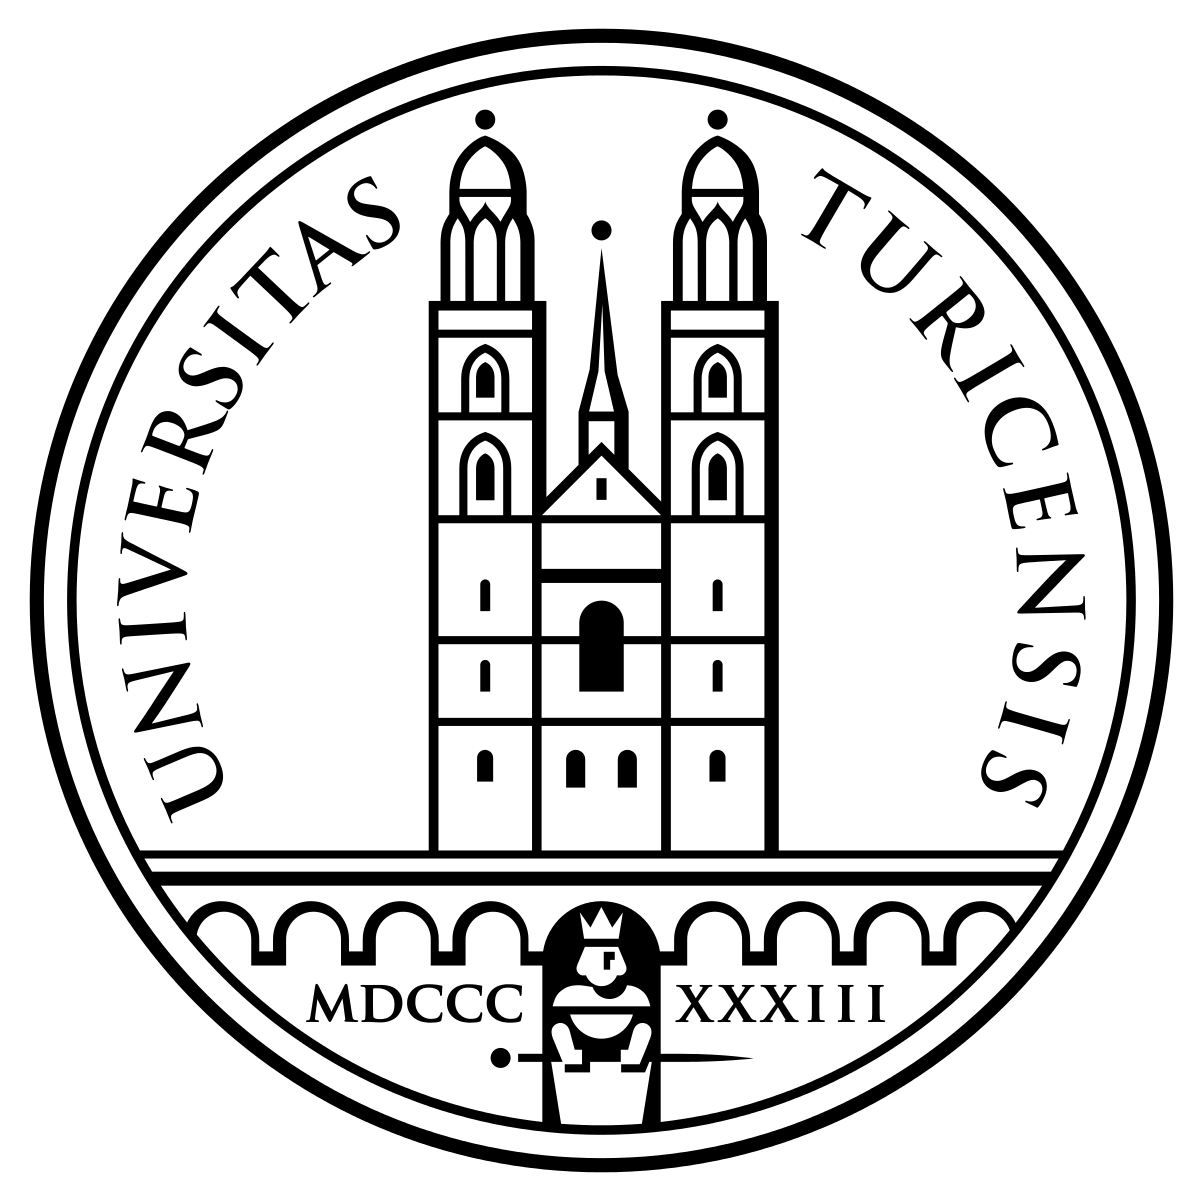
\includegraphics[width =0.34\textwidth]{UZH2.png}\\[1.2 cm]
      \textsc{\Large \textsc{Bachelorthesis}}\\[0.5 cm]

    \rule{\linewidth}{0.3 mm} \\[0.4cm]
    { \Large \bfseries Emergent Black Hole Dynamics in 1D and 2D Critical Floquet Systems}\\[0.3 cm]
    \rule{\linewidth}{0.3 mm} \\[1.5 cm]

  
    {\Large Fabian Jaeger}\\[2 cm] 
    
    
    		University of Zurich \\
             \textsc{Institute of Theoretical Physics} \\[1.5cm]
        
             	
    
    
    {\textbf{Supervised by}} \\[0.2cm]
   {\large  Prof. Dr. Titus Neupert} \\[2cm]
    
    {\large \today}\\[2 cm]
 
    \vfill
%    
%      \begin{minipage}{0.4\textwidth}
%        \begin{flushleft} \large
%            \textbf{Student}\\
%            \theauthor
%            \end{flushleft}
%            \end{minipage}~
%            \begin{minipage}{0.4\textwidth}
%            \begin{flushright} \large
%            \textbf{Enrollment Number} \\
%            17-740-325                                   % Your Student Number
%        \end{flushright}
%    \end{minipage}\\[1.2 cm]
    
\end{titlepage}

\begin{abstract}
    abstract-text
\end{abstract}

\newpage
\tableofcontents
\newpage

% ALl of the eigenstates and energy eigenvalues of a free fermion system can be obtained from anti-commuting algebra of the fermion operators.

	\section{Introduction}
	
	\section{Theory}
	
	\subsection{Tight-Binding Approximation}
	
	The energy structure of crystals depends on the interactions between orbitals in the lattice. The tight binding approximation neglects interactions between atoms separated by large distances. The tight-binding model calculates the electronic band structure using an approximate set of wave functions based upon superposition of orbitals located at each individual atomic site (LCAO).
	
	Considering Free Fermions with the Hamiltonian:
	\begin{equation}
		\hat{H}_\text{free} = \sum_{i,j} t_{ij} \hat{c}_i^\dagger \hat{c}_j
	\end{equation}
	with the hopping amplitude
	\begin{equation}
		t_{ij} = \frac{1}{N} \sum_{\vc{k}} \epsilon_{\mathbf{k}}^\text{free} e^{i \mathbf{k}\cdot (\mathbf{r}_i - \mathbf{r}_j)}
	\end{equation}
	The operatorproduct $\hat{c}_i^\dagger \hat{c}_j$ annihilates an electron on site $\mathbf{r}_j$ and creates one on site $\mathbf{r}_i$, which is what we coin as "hopping" from $\mathbf{r}_i$ to $\mathbf{r}_j$. In this sense the above Hamiltonian is a kinetic energy of the electron. \\
	

	In the tight-binding approximation we assume that:
	\begin{equation}
		t_{ij} = \begin{cases}
 			-t, \quad \text{if $i$ and $j$ are nearest neighbors} \\
 			0, \quad \text{otherwise}
		 \end{cases}
	\end{equation}
	meaning for a Bravais lattice we obtain the following tight-binding Hamiltonian
	\begin{equation}
		\hat{H}_{\text{tb}} = - t \sum_{\expval{ij}} ( \hat{c}_{i}^\dagger \hat{c}_j + \hat{c}_j^\dagger \hat{c}_i) = -\frac{t}{2} \sum_{i}\sum_{\vc{\delta}} (\hat{c}_i^\dagger \hat{c}_{i + \vc{\delta}} + \hat{c}_{i + \vc{\delta}} \hat{c}_i)
	\end{equation}
	where in the second step we expanded the nearest neighbor sum $\expval{ij}$ and inserted the 1/2 to avoid double counting. The sum $\sum_{\vc{\delta}}$ sums over all the nearest neighbor vectors of $\vc{\delta}_1, \vc{\delta}_2, \dots \vc{\delta}_q$. In my work (as we will not consider diagonal hopping for $d \geq 2$) we simply have $q = 2d$ where $d$ is the dimension of the Bravais lattice. \\
	
	Solving the Hamiltonian includes finding the eigenvalues and eigenvectors of this matrix. However for the case of translational-invariance which corresponds to periodic-boundary conditions, i.e $\hat{c}_{i + La}^\dagger = \hat{c}_i$, the Hamiltonian is diagonalizing simply with the use of the anticommutator rules for fermions. For this we consider a change of basis to the momentum space representation. A change of Basis for a second-quantised operator is given by
	\begin{equation}
		\hat{c}_\alpha^\dagger = \sum_\beta \braket{\beta}{\alpha} \hat{c}_\beta^\dagger \qq{and} \hat{c}_\alpha = \sum_\beta \braket{\alpha}{\beta} \hat{c}_\beta
	\end{equation}
	where $\{\ket{\alpha}\}$ and $\{\ket{\beta}\}$ are a full set of orthonormal basis states that span the Hilbert space. A projection onto momentum space from our position-set $\{\ket{j}\}$
		\begin{equation}
		\braket{\mathbf{k}}{j} = \psi_{\mathbf{k}}^*(\mathbf{r}_j) = \frac{1}{\sqrt{N}} e^{-i \mathbf{k} \cdot \mathbf{r}_j} \qq{and} \braket{j}{\mathbf{k}} = \psi_\mathbf{k}(\mathbf{r}_j) = \frac{1}{\sqrt{N}} e^{i \mathbf{k} \cdot \mathbf{r}_j}
	\end{equation}
	results in the creation and annihilation operator in momentum space:
	\begin{equation}
		\hat{c}_{\mathbf{k}} = \frac{1}{\sqrt{N}}  \sum_{\mathbf{k}} e^{-i \mathbf{k}\cdot \mathbf{r}_j} \hat{c}_{\mathbf{k}}^\dagger \qq{and} \hat{c}_\mathbf{k} = \frac{1}{\sqrt{N}} \sum_\mathbf{k} e^{i \mathbf{k} \cdot \mathbf{r}_j} \hat{c}_\mathbf{k}
	\end{equation}
	which inverted yields us:
	\begin{equation}
		\hat{c}_j = \frac{1}{\sqrt{N}} \sum_k e^{i \mathbf{k}\cdot \mathbf{r}_j} \hat{c}_\mathbf{k} \qq{and} \hat{c}_j^\dagger = \frac{1}{\sqrt{N}} \sum_k e^{-i\mathbf{k}\cdot \mathbf{r}_j} \hat{c}_\mathbf{k}^\dagger
	\end{equation}
	For the Hamiltonoperator we therefore have
	\begin{equation}
		\hat{H}_0 = \frac{1}{2}\sum_{j=1}^{L-1}  \hat{c}_j^\dagger \hat{c}_{j+1} +\hat{c}_{j+1}^\dagger \hat{c}_j = \frac{1}{2N}\left[ \right]
	\end{equation}
	The unperturbed Hamiltonian $H_0$ is diagonal in the momentum-space representation and can be written as
	\begin{equation}
		\hat{H}_0 = \sum_k \epsilon_k \hat{c}_k^\dagger \hat{c}_k
	\end{equation}
	with $\varepsilon_k$ being the single particle energy associated with the wave vector $k$. The ground state of such a system is the Fermi sea with
	\begin{equation}
		\ket{G} = \prod_{k \in \text{occ}} \hat{c}_k^\dagger \ket{0}
	\end{equation}
		In our models we will disregard the spin of the particles and therefore a maximum of one electron is allowed to occupy a given lattice site at any given time due to the Fermi-Dirac Statistics. It follows that for the ground state $\ket{G}$ of $\hat{H}_0$:
	\begin{equation}
	\begin{split}
		\hat{c}_k \ket{G} = 0, \qq{if} \epsilon_k > 0 \\
		\hat{c}_k^\dagger \ket{G} = 0, \qq{if} \epsilon_k < 0
 	\end{equation}

	
	

	
	\subsubsection{Exact Solution for PBC}
		
	
	
	\subsubsection{One-dimensional free-fermion Lattice}
	
	The Operatorproduct $\hat{c}_i^\dagger \hat{c}_{j}$ annihilates a fermion at position $x = ia$ where $a$ is the Lattice constant and creates one in at the position $x= ja$. This "hopping" can be visualized as following. In our approximations we will restrict ourselves to nearest-neighbor hopping meaning we simply consider the simplified tight-binding Hamiltonian:
	\begin{equation}
		\hat{H}_0 = \frac{1}{2} \sum_i^{L-1} \hat{c}_i \hat{c}_{i+1} + \hat{c}_{i+1}^\dagger \hat{c}_i
	\end{equation}
	For a 1-Dimensional Lattice of $N$ sites the Hamiltonian $\hat{H}_0$ is a $N \times N$ matrix. The Hilbert space $\mathcal{H}_0$ has $N$ states. 	
	
	
	\begin{figure}[h]
		\centering
		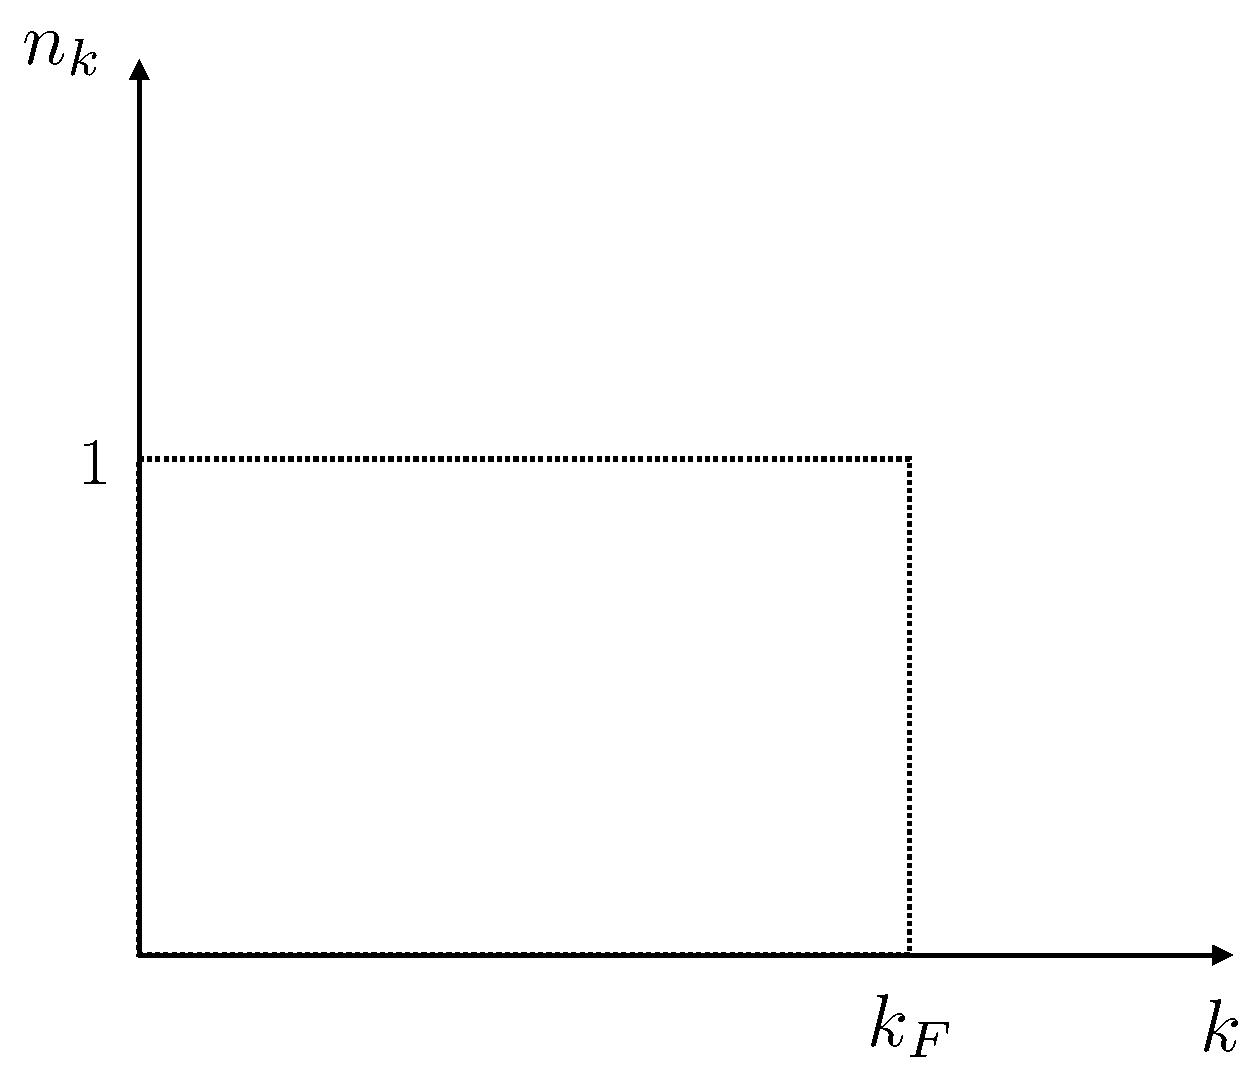
\includegraphics[width=0.8\textwidth]{Disperion_relation1D}
		\caption{Dispersion relation and Occupation for a free fermion system (without spins) in one-dimension}
	\end{figure}
	
	\subsubsection{Two-dimensional Tight-binding system}
	Here we wish to consider a square lattice with Lattice constant $a$ in both directions. Each Electron has 4 neighboring sites
	
	\begin{figure}[h]
		\centering
		\begin{subfigure}[t]{0.49\textwidth}
		\centering
			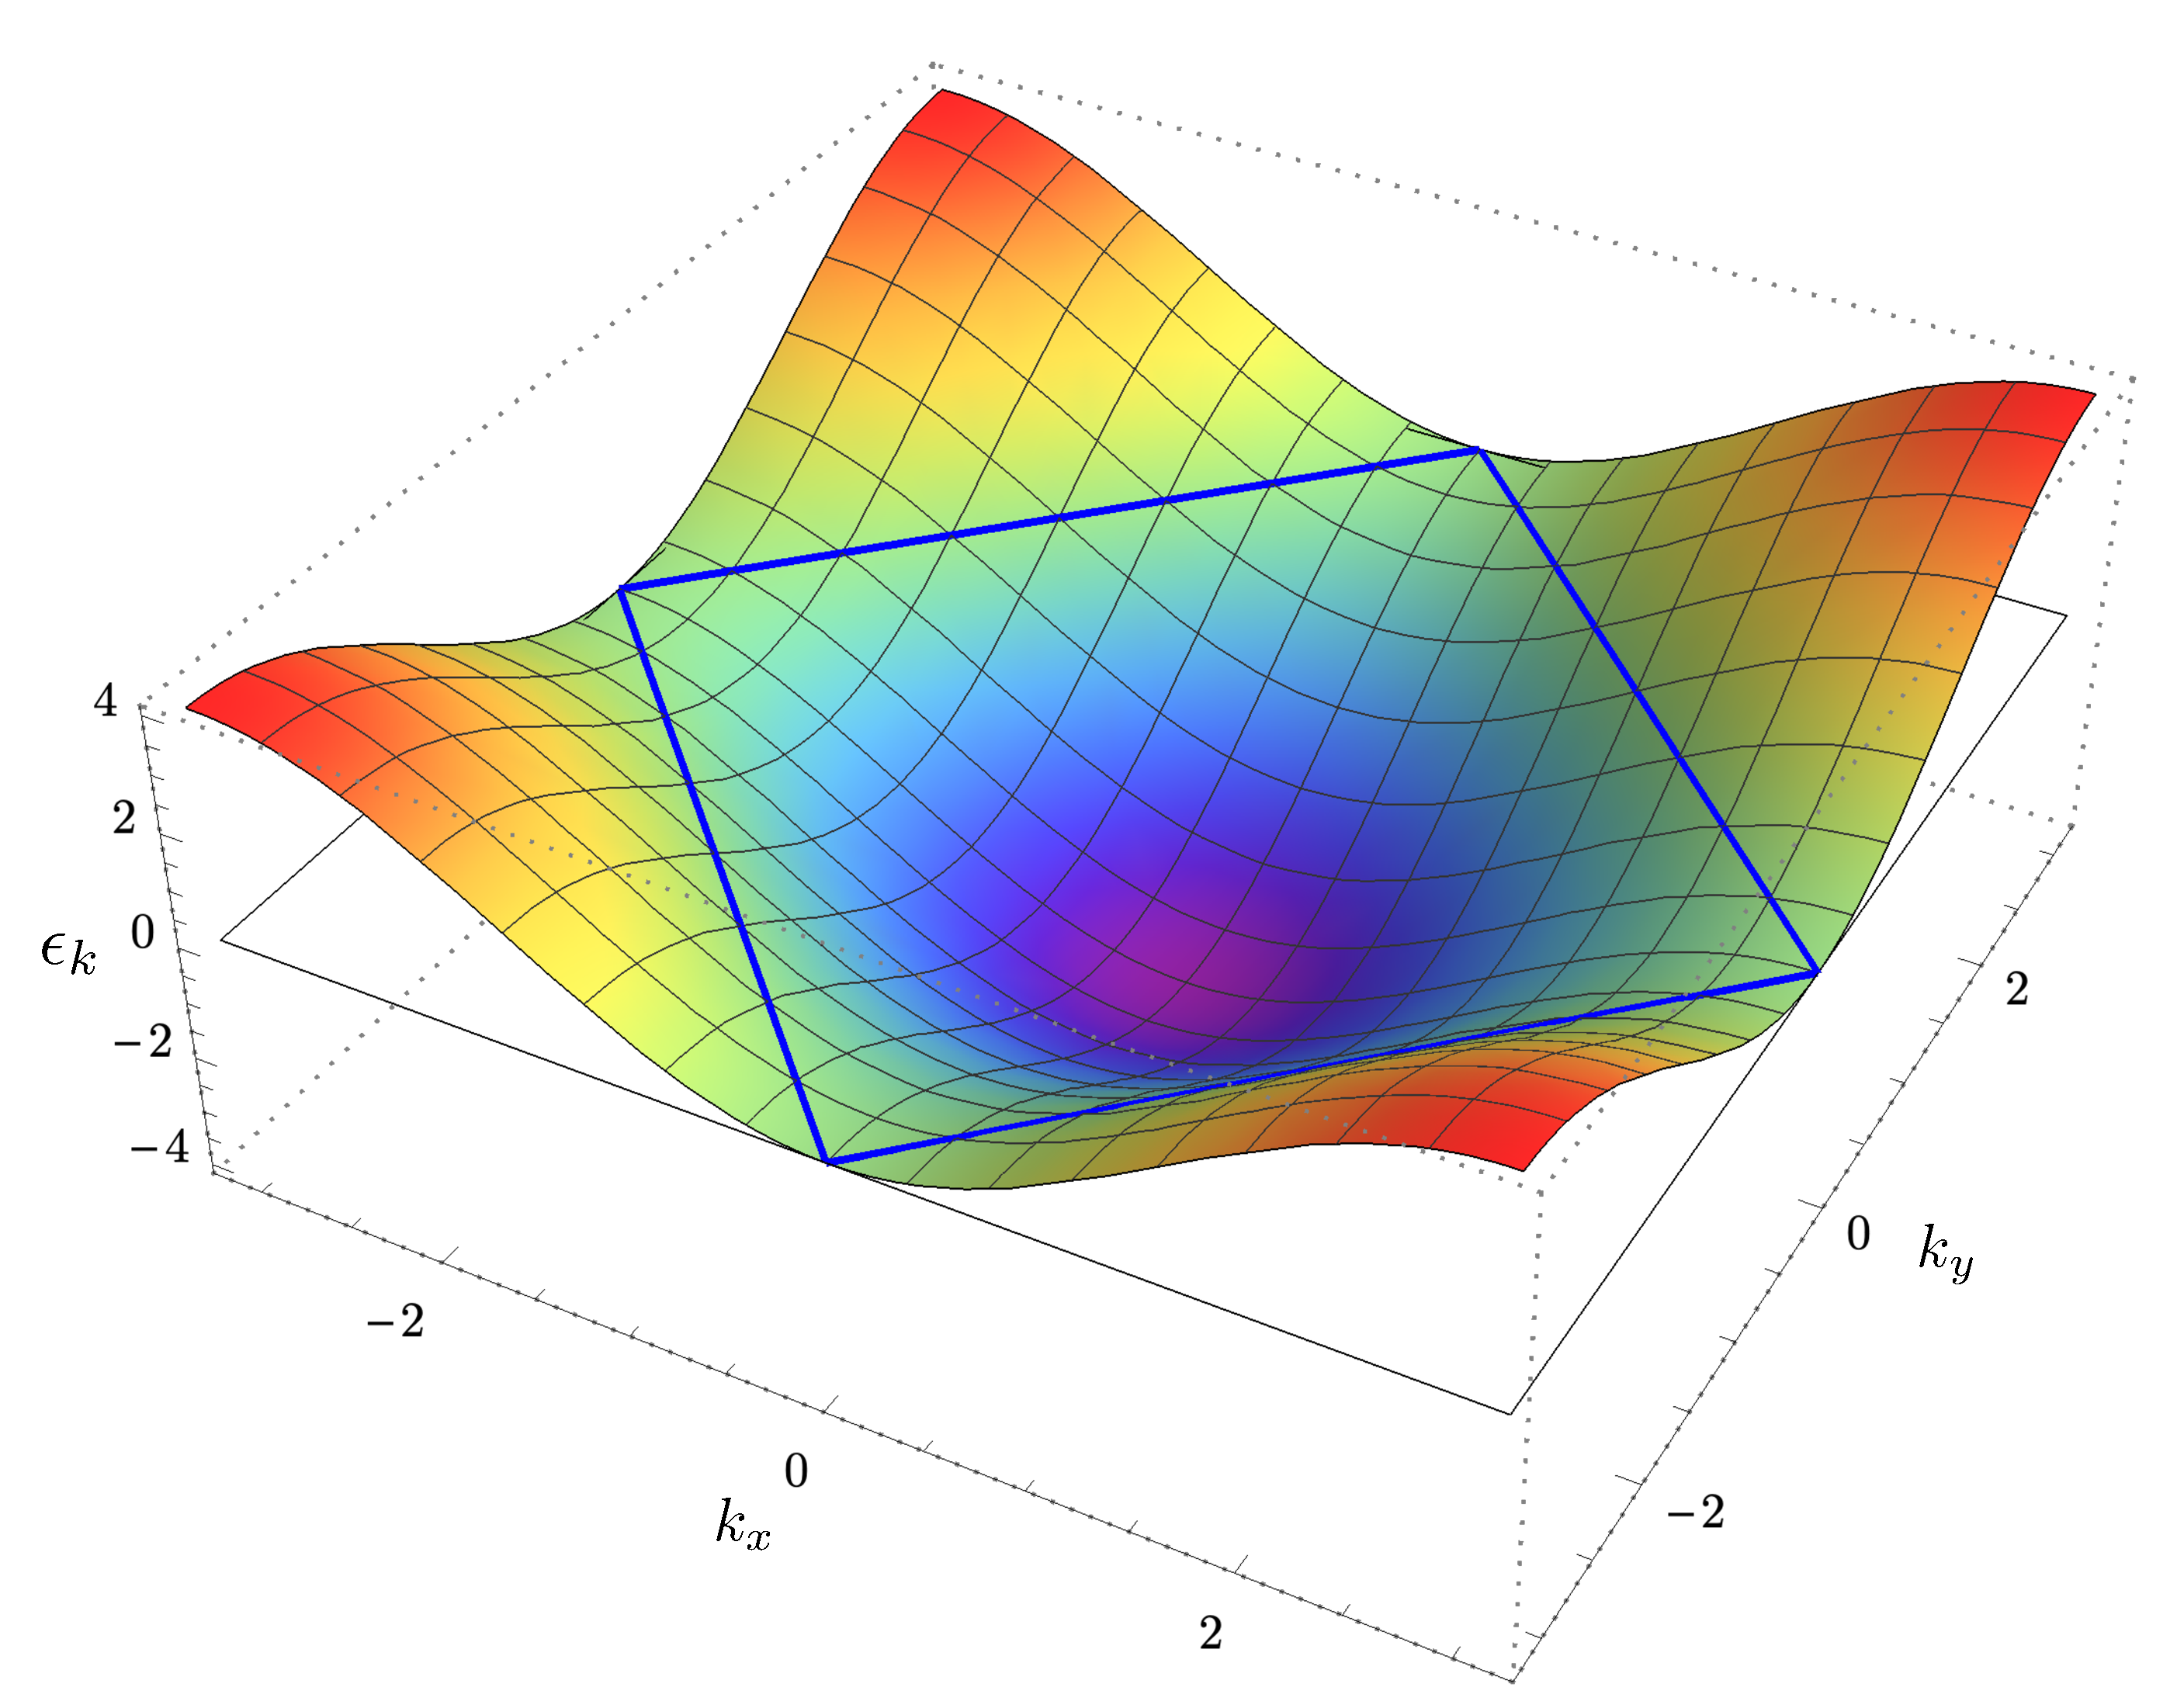
\includegraphics[width =\textwidth]{Dispersion_relation2d}
			\caption{}
		\end{subfigure}
		\begin{subfigure}[t]{0.49\textwidth}
		\centering
			\includegraphics[width =0.8\textwidth]{Dispersion_Relation2d_Top}
			\caption{}
		\end{subfigure}
		\caption{Dispersion Relation for a 2D tight binding Hamiltonian; (a) Dispersion relation for the tight binding Hamiltonian in two-dimensions. Up to the blue lines around the Energy $\epsilon_k = 0$ the states are filled in the ground state. The Fermi surface separates the occupied states from the non-occupied ones. Here displayed is the first brillouin zone}
	\end{figure}
	
	\subsection{Sine-Squared Deformed Hamiltonian}
	
	
	
	
	The reason Sine-Squared deformation Hamiltonians are studied is because in Conformal Field Theory they can exactly be solved. This extends also to Floquet CFT. For the Sine squared Hamiltonian the binding strength towards the middle of the chain is stronger than on the edges. 
	% Explanation as to why use the sine-squared deformed Hamiltonian -> See paper Sine-square deformation of free fermion system
	
	\subsection{Floquet System}
	In this we will consider a free fermion chain with half filling:
	\begin{equation}
	\hat{H}(t) = 
		\begin{dcases}
		\hat{H}_0 = \frac{1}{2} \sum_{i=1}^{L-1} (\hat{c}_i^\dagger \hat{c}_{i+1} + \hat{c}_{i+1}^\dagger \hat{c}_{i})\\
		\hat{H}_\text{SSD} = \sum_{i=1}^{L-1} \sin^2\left( \frac{\pi(i + 1/2)}{L}\right) \left[ \hat{c}_i^\dagger c_{i+1} + \hat{c}_{i+1}^\dagger \hat{c}_i \right]
		\end{dcases}
	\end{equation}
	The factor $1/2$ is there to avoid double counting.
	with $\hat{c}_i$ and $\hat{c}_{i+1}^\dagger$ fermionic operators which satisfy the fermionic anticommutation relation
	\begin{equation}
		\{ \hat{c}_i, \hat{c}_j\} = \{\hat{c}_i^\dagger, \hat{c}_j^\dagger\} = 0 \qq{and} \{ \hat{c}_i, \hat{c}_j^\dagger \} = \delta_{ij}
	\end{equation}
	In our models we will disregard the spin of the particles and therefore a maximum of one electron is allowed to occupy a given lattice site at any given time due to the Fermi-Dirac Statistics. It follows that for the ground state $\ket{G}$ of $\hat{H}_0$ \\

	
	At $t=0$ we prepare the initial state as the ground state $\ket{G}$ of $\hat{H}_0$. We switch and alternate this driving procedure in time by switching between the two different Hamiltonians. This procedure is pictorially illustrated in the figure
\begin{figure}[h]
\centering
		\begin{subfigure}[b]{0.45\textwidth}
			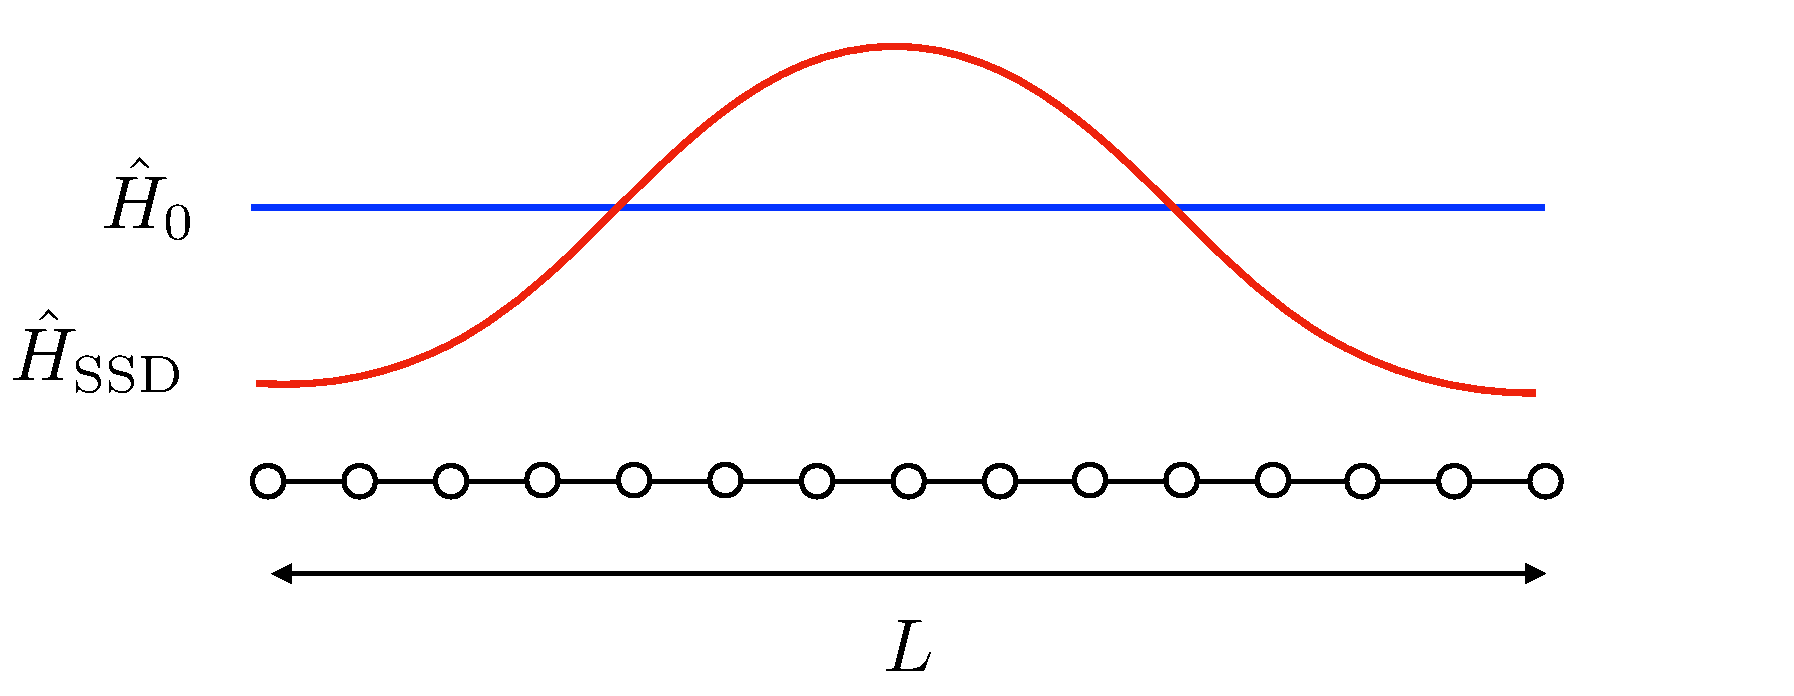
\includegraphics[width=\textwidth]{Floquet_Drive1D_Deformation.pdf}
			\caption{}
		\end{subfigure}
		\begin{subfigure}[b]{0.45\textwidth}
			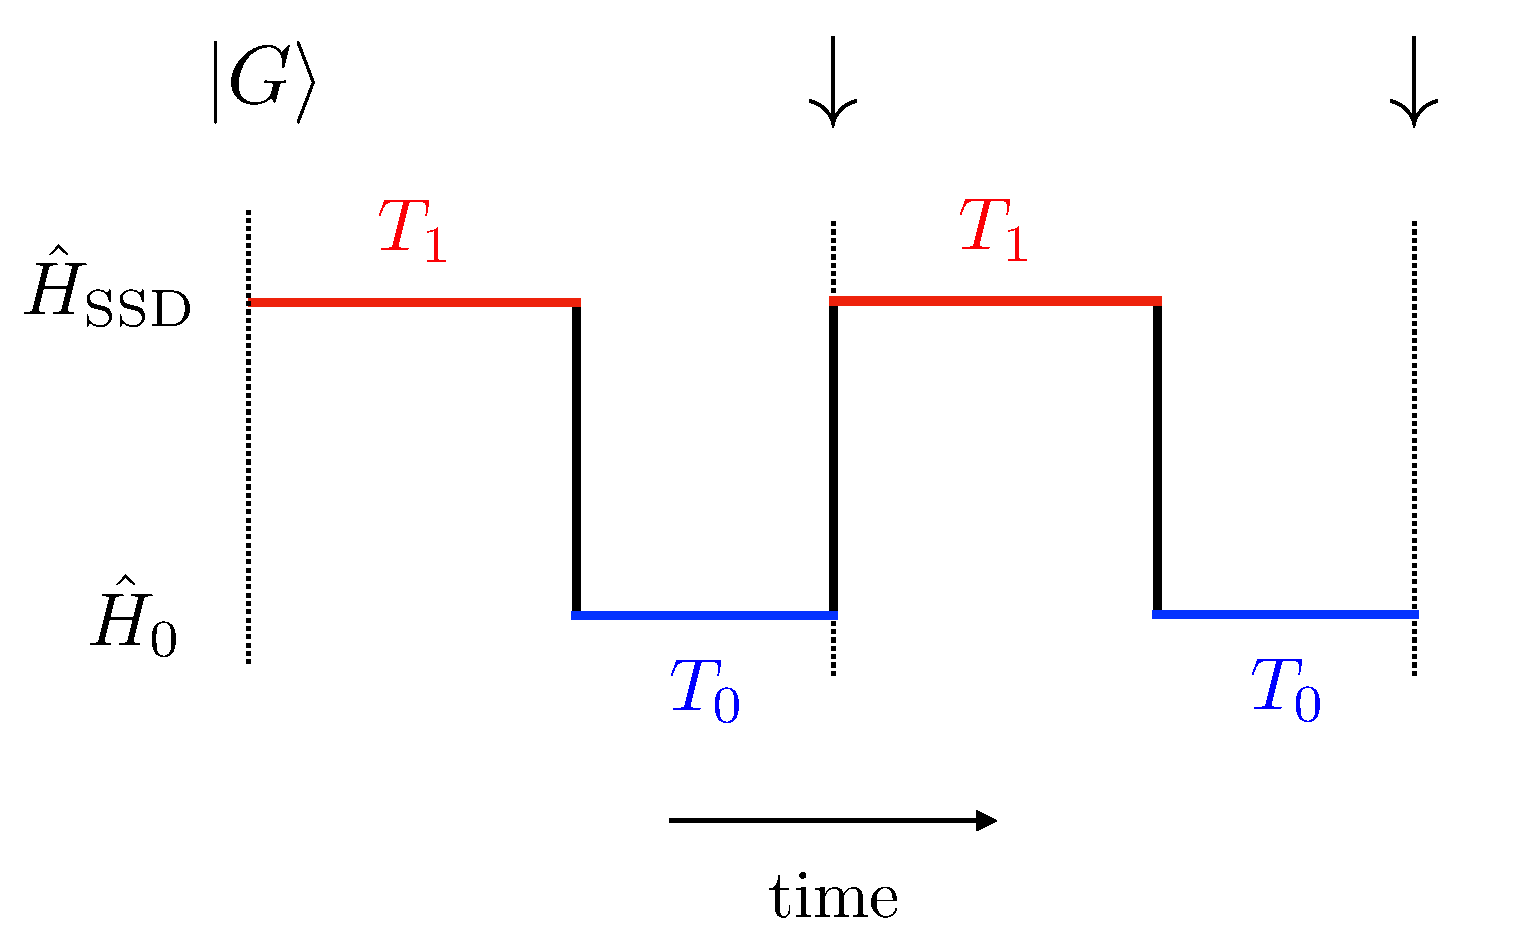
\includegraphics[width=0.95\textwidth]{Floquet_Drive.pdf}
			\caption{}
		\end{subfigure}
		\caption{(a) Hamilton Densities for the tight-binding Hamiltonian and SSD deformation (b) Floquet driving where the black arrow indicate stroboscopic measurement}
\end{figure}
	Our initial state is the ground state of the Hamiltonian $\hat{H}_0$. In the following steps we then apply the Hamiltonian $\hat{H}_1$ to $\ket{G}$ followed by $\hat{H}_0$. This procedure is repeated in time, where the evolution from the Ground state $\ket{G}$ in terms of the Hamiltonian $\hat{H}_1$ is given by the unitary time evolution operator:
	\begin{equation}
		\ket{\psi_1(t)} = \hat{U}\ket{G} = \exp(-\frac{i}{\hbar} \hat{H}_1 t)\ket{G}
	\end{equation} 
	The main computational work will involve computing the two-point correlation functions that will allow us to study the properties of the Floquet dynamics of the system. \\
	
	We initialize the system in the ground state $\ket{G}$ of the Hamiltonian $\hat{H}_0$. In a stroboscopic measurement, the Floquet dynamics is determined by the state 
	\begin{equation}
		\ket{\psi(nT)} = \hat{F}^n \ket{G} \qq{with} \hat{F} = e^{-i \hat{H}_0 T_0} e^{i \hat{H} T_1}
	\end{equation}
	
	The two-point correlation function of local operators $\hat{\mathcal{O}}_1(x_1)$ and $\hat{\mathcal{O}}(x_2$ after $n$-cyles is given by
	\begin{equation}
		\mathcal{C}_{ij}
	\end{equation}
	In the Heisenberg picture, the calculation amounts to determining the operator evolution $\hat{\mathcal{O}}(x, nT) = F^{-n} \hat{\mathcal{O}}(x) F^{n}$. For a general Floquet drive computing this time evolution is a non-trivial task. However for the simple case of a tight-binding-approximation and its sine-squared deformation it not-only has a precise treatment in Conformal Field Theory but the numerical calculation is furthermore fairly straight forward.
	
	\section{Floquet Theory and the Floquet theorem}
	(Topological Floquet System)

	Floquet Theory investigates quantum systems of periodic Hamiltonians in time: 
	\begin{equation}
		\hat{H}(t) = \hat{H}(t+ T)
	\end{equation}
	where $T$ is the period of perturbation. In our example this will simply be the period of driving the SSD Hamiltonian. Floquet theory also requires the condition of linearity which in the case of the Schrödinger-equation is inherently satisfied (Since the Schrödingerequation is linear). We know that the dynamics of a quantum mechanical System can be described by two completely analogous procedures, with the time-dependent Schrödingerequation
	\begin{equation}
		i\hbar \dv{t} \ket{\psi(t)} = \hat{H}(t) \ket{\psi(t)}
	\end{equation}
	or with the use of the unitary time evolution operator $\hat{U}(t,t_0)$:
	\begin{equation}
		\ket{\psi(t)} = \hat{U}(t,t_0) \ket{\psi(t_0)}
	\end{equation}
	Now in our case we will not simply be considering the evolution in terms of the Hamiltonian $\hat{H}_0$ but also $\hat{H}_1$. In the general case in which the different Hamiltonians at different times do not commute with each other $\comm*{\hat{H}(t)}{\hat{H}(t')} \neq 0$ is not a simple exponential product but rather a time-ordered series which can broadly be categorized as a Dyson expansion. 
	\begin{align}
	\hat{U}(t,t_0) &= \textup{T} \exp(	-\frac{i}{\hbar} \int_{t_0}^t \dd t' \hat{H}(t'))\\
	&= \mathbbm{1} + \left(- \frac{i}{\hbar}\right) \int_{t_0}^t \dd t_1 \hat{H}(t_1) + \left(-\frac{i}{\hbar}\right)^2 \int_{t_0}^t \dd t_1 \hat{H}(t_1) \int_{t_0}^{t_1} \dd t_2 \hat{H}(t_2) + \dots
	\end{align}
	where $\textup{T}$ stands for the time-ordered product, meaning that for the $n$-th term in the expansion we have a ordered product of $\hat{H}(t_1)\hat{H}(t_2)\dots \hat{H}(t_n)$ of non-commuting Hamiltonians\\
	
	
With the condition of periodicity as is the case for Floquet Hamiltonians we aim to show that the time-evolution operator can however be factorised according to
	\begin{equation}
		\hat{U}(
	\end{equation}
	This will not be relevant for us since we will consider piecewise constant Hamiltonians in time, meaning we can simply consider a 
	
	\section{Theoretical Framework}
	The main goal of this thesis was to establish the entanglement entropy and Energy density of a free fermion lattice under Floquet driving. As we will explicitly show these two quantities can be evaluated with the help of the equal time two-point correlation functions.

	\subsection{Ground State}
	To obtain the matrix form of the Hamiltonian operator $\hat{H}_0$ in the ground state we need to evaluate the correlation matrix
	\begin{equation}
		\mel{G}{\hat{H}_0}{G}
	\end{equation}
	In general this resulting matrix is not diagonal. Our goal is to find a Basistransformation of the creation- and annihiliation operators $\hat{c}$ that will diagonalise $\hat{H}_0$, i.e
	\begin{equation}
		\hat{H}_0 = \sum_{i=1}^L E_i^{(0)} \hat{a}_i^\dagger \hat{a}_i
	\end{equation}
	where the operators once again fullfill the fermionic anticommutation rules
	\begin{equation}
		\{ \hat{a}_i,\hat{a}_j^\dagger \} = \delta_{ij} \qq{and} \{\hat{a}_i^\dagger, \hat{a}_j^\dagger\} = \{\hat{a}_i,\hat{a}_j  \} =0
	\end{equation}
	It is know that a general one-particle operator in second quantized form takes the shape
	\begin{equation}
		\hat{A} = \sum_{\mu, \nu} \mel{\nu}{\hat{A}}{\mu} \hat{a}_\nu^\dagger \hat{a}_\mu
	\end{equation}
	meaning for our Operator in the Ground state we have to evaluate
	\begin{equation}
		\hat{H}_0 = \sum_{n, m} \mel{m}{\hat{H}_0}{n} \hat{c}_m^\dagger \hat{c}_n
	\end{equation}
	Our Goal is it to find an orthogonal matrix representation of this operator. For this note that if $H_{mn} = \mel{m}{\hat{H}_0}{n} = E_n^{(0)} \delta_{mn} $ with the energy-eigenstates $E_n^{(0)}$ of the Hamiltonoperator $\hat{H}_0$ we obtain the diagonal matrix form
	\begin{equation}
	\hat{H} = 
	\begin{pmatrix}
 		\mel{1}{\hat{H}_0}{1} & \mel{1}{\hat{H}_0}{2} & \dots & \mel{1}{\hat{H}_0}{L} \\
 		\mel{2}{\hat{H}}{1} & \ddots &\dots \\
 		\vdots & \dots & \ddots & \vdots \\
 		\mel{L}{\hat{H}}{1}
 	\end{pmatrix}
	\end{equation}
	Our goal is therefore to evaluate the following expressions
	\begin{equation}
		H_{mn} = \mel{\varphi_m}{\hat{H}_0}{\varphi_n} = \mel{0}{\hat{c}_m\hat{H}_0 \hat{c}_n}{0}
	\end{equation}
	where we used the single-particle Basisstates $\{\varphi_m\}$ and the fact that for fermions we can only occupy one particle for each state.
	Inserting the expression for our Hamiltonoperator 
	\begin{equation}
		\hat{H}_0 = \frac{1}{2} \sum_{i=1}^{L-1} \hat{c}_i^\dagger \hat{c}_{i+1} + \hat{c}_{i+1}^\dagger \hat{c}_{i} 
	\end{equation}
	we get
	\begin{align}
	H_{mn}^{(0)} = \frac{1}{2}\sum_{i=1}^{L-1}\mel{0}{\hat{c}_m \left[ \hat{c}_i^\dagger \hat{c}_{i+1} + \hat{c}_{i+1}^\dagger \hat{c}_i\right]\hat{c}_n^\dagger}{0} = \frac{1}{2}\sum_{i=1}^{L-1} \mel{0}{\hat{c}_m \hat{c}_i^\dagger \hat{c}_{i+1} \hat{c}_n^\dagger}{0} + \mel{0}{\hat{c}_m \hat{c}_{i+1}^\dagger \hat{c}_i\hat{c}_n^\dagger}{0}
	\label{eq:Energy_Density_Matrix}
	\end{align}

	
	 However it is known that with a unitary similarity transformation we can reduce it into a diagonal form. For the two terms it follows from Wick's theorem that with the help of contractions we can express any expectation value of Matrix element in terms of the action on the vacuum state $\ket{0}$:
	 \begin{itemize}
	 	\item For the first term in the expression, we obtain
	 	\begin{align}
	 		\sum_i \mel{0}{\hat{c}_m \hat{c}_{i}^\dagger \hat{c}_{i+1} \hat{c}_n^\dagger}{0} &= \sum_i \mel{0}{\hat{c}_m \hat{c}_i^\dagger (\delta_{i +1, n} - \hat{c}_n^\dagger\hat{c}_{i+1})}{0}\\
	 		 &= \sum_i \delta_{i+1, n} \mel{0}{\hat{c}_m \hat{c}_i^\dagger}{0} - \mel{0}{\hat{c}_m \hat{c}_i^\dagger \hat{c}_n^\dagger\hat{c}_{i+1}}{0}
	 		 \label{eq:secondterm2}
	 	\end{align}
	 	where in the second step we used the anticommutator relation for the creation and annihilation operators:
	 	\begin{equation}
	 		\{ \hat{c}_{i+1}, \hat{c}_n^\dagger \} = \hat{c}_{i+1} \hat{c}_n^\dagger + \hat{c}_n^\dagger\hat{c}_{i+1} \; \Rightarrow \; \hat{c}_{i+1} \hat{c}_n^\dagger = \underbrace{\{ \hat{c}_{i+1}, \hat{c}_n^\dagger \}}_{\delta_{i+1, n}} - \hat{c}_n^\dagger \hat{c}_{i+1}
	 		\label{eq:Kommutatorrelation_umgeformt}
	 	\end{equation}
	 	Noting that the second term in (\ref{eq:secondterm2}) is zero due to $\hat{c}_{i+1}\ket{0} =0$ and that with
	 	\begin{equation}
	 		\hat{c}_m \hat{c}_{i}^\dagger = \underbrace{\{ \hat{c}_m, \hat{c}_i^\dagger\}}_{\delta_{m, i}} - \hat{c}_i^\dagger \hat{c}_m
	 	\end{equation}
	 	in analogy to (\ref{eq:Kommutatorrelation_umgeformt}) we finally obtain the expression
	 	\begin{equation}
	 		\mel{0}{\hat{c}_m \hat{c}_i^\dagger \hat{c}_{i+1}\hat{c}_n^\dagger}{0} = \sum_i \delta_{i+1,n}\delta_{m, i} =\delta_{m, n-1}
	 		\label{eq:first_term_correlation_matrix}
	 	\end{equation}
	 	where we again used $\hat{c}_m \ket{0} = 0$ meaning $\mel{0}{\hat{c}_i^\dagger \hat{c}_m}{0} = 0$.
	 	 \item For the second term in the expression, we proceed analogously to above. For completeness it is nonetheless repeated here. \begin{align}
	 		\sum_i \mel{0}{\hat{c}_m \hat{c}_{i+1}^\dagger \hat{c}_{i} \hat{c}_n^\dagger}{0} &= \sum_i \mel{0}{\hat{c}_m \hat{c}_{i+1}^\dagger \left( \delta_{i,n} - \hat{c}_n^\dagger \hat{c}_i \right)}{0} \\
	 		&=  \sum_i \delta_{i,n}\mel{0}{\hat{c}_m \hat{c}_{i+1}^\dagger }{0} - \underbrace{\mel{0}{\hat{c}_m \hat{c}_{i+1}^\dagger \hat{c}_n^\dagger\hat{c}_{i+1}}{0}}_{=0}
	 	\end{align}
	 	Using $\hat{c}_m \hat{c}_{i+1}^\dagger = \delta_{m, i+1} - \hat{c}_{i+1}^\dagger \hat{c}_m$ and the fact that $\mel{0}{\hat{c}_{i+1}^\dagger \hat{c}_m}{0} = 0$ we obtain
	 	\begin{equation}
	 		\sum_i \mel{0}{\hat{c}_m \hat{c}_{i+1}^\dagger \hat{c}_i \hat{c}_n^\dagger}{0} = \sum_{i} \delta_{i,n} \delta_{m, i+1} = \delta_{m, n+1}
	 		\label{eq:second_term_correlation_matrix}
	 	\end{equation}
	 \end{itemize}
	 With (\ref{eq:second_term_correlation_matrix}) and (\ref{eq:first_term_correlation_matrix}), it follows that our Hamiltonoperator $\hat{H}_0$ we obtain the bi-diagonal form:
	 \begin{equation}
	 	H^{(0)}_{mn} = \frac{1}{2} \left(\delta_{m, n+1} + \delta_{m+1, n}\right)
	 \end{equation}
	 It can analogously be shown, that for the Hamiltonian $\hat{H}_1$ we obtain following Matrixelements
	 \begin{equation}
	 	H_{mn}^{(\text{SSD})} = \sin^2\left(\frac{\pi(n-1/2)}{L}\right) \delta_{m,n-1} + \sin^2\left(\frac{\pi(n+1/2)}{L}\right) \delta_{m,n}
	 \end{equation}
	 It is clear that the two-point Correlation Matrix is not diagonal in the single-particle Basis set $\{ \varphi_i \}$. To diagonalize the matrix we consider a change of basis to some other single-particle basis set $\{\psi_j\}$ with
	 \begin{equation}
	 	\hat{a}_j = \sum_i \braket{\psi_j}{\varphi_i} \hat{c}_i \qq{and} \hat{a}_j^\dagger =\sum_i \braket{\varphi_i}{\psi_j} \hat{c}_i^\dagger
	 \end{equation}
	 If we let $U_{i,j} = \braket{\varphi_i}{\psi_j}$ be the matrix elements of the unitary transformation we can compactly write
	 \begin{equation}
	 	\hat{a}_j = \sum_i (U^\dagger)_{ji} \hat{c}_i \qq{and} \hat{a}_j^\dagger = \sum_i (U^\dagger)^*_{ji} \hat{c}_i^\dagger =\sum_{i}  \hat{c}_i^\dagger U_{ij}
	 \end{equation}
	 
	 
	 
	 where we used $U_{ij}^* = (U^\dagger)_{ji}$. To show that the transformation matrix is indeed unitary, consider
	 \begin{align}
	 	\delta_{j,k} &= \braket{\psi_j}{\psi_k} = \sum_i \braket{\psi_j}{\varphi_i}\braket{\varphi_i}{\psi_k} = \sum_i \braket{\varphi_i}{\psi_j}^* \braket{\varphi_i}{\psi_k} \\
	 	&= \sum_i U_{ij}^* U_{ik} = \sum_i (U^\dagger)_{ji} U_{ik} = (U^\dagger U)_{jk} \quad \Rightarrow \quad U^\dagger U = \mathbbm{1}
	 \end{align}
	 The inverse of this transformation yields
	 \begin{equation}
	 	\hat{c}_n = \sum_i U_{ni} \hat{a}_i \qq{and} \hat{c}_n^\dagger = \sum_i \hat{a}_i^\dagger U^*_{ni} = \sum_i \hat {a}_i^\dagger (U^\dagger)_{in}
	 \end{equation}
	 It is well known that any hermitian matrix $A$ is diagonalizable by an appropriate unitary similarity transformation
	 \begin{equation}
	 	U^\dagger A U = \begin{pmatrix}
	 		\lambda_1 & 0 &\dots & 0 \\
	 		0 & \lambda_2 & \dots & 0 \\
	 		\vdots & \vdots & \ddots & \vdots \\
	 		0 & 0 & \dots & \lambda_n
	 	\end{pmatrix}
	 \end{equation}
	 where $\lambda_1, \dots \lambda_n$ are the eigenvectors of the hermitian matrix $A$ and the columns of $U$ are spanned by the eigenvectors of the hermitian matrix $A$. By this given unitary transformation we can diagonalise the Hamiltonian:
	 \begin{equation}
	 	\hat{H}_0 = \sum_{i=1}^L E_i^{(0)} \gamma_i^\dagger \gamma_i = E_i^{(0)} \hat{n}_i
	 \end{equation}
	 where $\hat{n}_i$ denotes the fermionic occupation number operator at site $i$. In the case of translational invariance for the chain (i.e closed boundary conditions) a simple choice of unitary transformation would be transforming to the momentum basis (essentially using a Fourier transform). We simply want to consider a general case with open- or closed boundary conditions. Since we are considering a half-filled free fermion chain our ground state $\ket{G}$ in these new operators can be written as:
	 \begin{equation}
	 	\ket{\psi(0)} =\ket{G} = \prod_{i=1}^{L/2} \gamma_i^\dagger \ket{0}
	 \end{equation}
	 We note that in the case of periodic boundary conditions the operators $\hat{\gamma}_i, \hat{\gamma}_i^\dagger$ correspond to the operators $\hat{c}_k$ and $\hat{c}_k^\dagger$ respectively.

	\subsection{Quantum Quench and Floquet Case}
	This procedure follows closely the paper of Xueda Wen \\
	
	Our goal will be to find the two-point correlation function
	For a single quench  \cite{Xueda}
	After time $T_0$ has passed we now want to consider what happens to a single quench by evolving the ground state $\ket{G}$. Since $\hat{H}_\text{SSD}$ is time-independent it is well know that the time evolution of a state $\ket{\psi(t)}$ in the Schrödinger picture is given by applying the unitary evolution operator $\hat{U} = \exp(i\hat{H}_\text{SSD} t)$ on the ground state $\ket{\psi(t=0)} = \ket{G}$:
	\begin{equation}
		\ket{\psi(t)} = \exp(-i \hat{H}_1 t) \ket{G}
	\end{equation}
	We wish to evaluate the equal-time two-point correlation function:
	\begin{equation}
	\mathcal{C}_{m,n} = \mel{\psi(t)}{\hat{c}_m^\dagger \hat{c}_n}{\psi(t)}	
	\end{equation}
	\begin{equation}
		\mathcal{C}_{\mathcal{O}} = \expval{\hat{\mathcal{O}}} = \text{Tr}(\rho \hat{\mathcal{O}})
	\end{equation}
	The correlation function for our case not in thermale equilibrium is given by
	\begin{equation}
		 = \frac{1}{\operatorname{tr}\left(e^{-\beta H}\right)} \operatorname{tr}\left(c_{i}^{\dagger} c_{j} e^{-\beta H}\right)
	\end{equation}
Instead of working in the Schrödinger picture we want to work in the Heisenberg one. Therefore we consider
	\begin{equation}
		\mel{\psi(t)}{\hat{c}_m^\dagger \hat{c}_n}{\psi(t)} = \mel{G}{e^{i \hat{H}_1 t} \hat{c}_m^\dagger \hat{c}_n e^{-i \hat{H}_1 t}}{G} = \mel{G}{e^{i\hat{H}_1 t} \hat{c}_m^\dagger e^{-i \hat{H}_1 t} e^{i \hat{H}_1 t} \hat{c}_n e^{-i\hat{H}_1 t}}{G}
		\label{eq:Correlation_Matrix_singlequench}
	\end{equation}
	Where in the second equality we inserted the expression $\hat{U}^\dagger \hat{U} = \exp(i \hat{H}_1 t)\exp(-i \hat{H}_1 t) = \mathbbm{1}$. Our goal will be to simply the two expressions:
	\begin{equation}
		\bra{G} e^{i\hat{H}_1 t} \hat{c}_m^\dagger e^{-i \hat{H}_1 t} \qq{and}  e^{i \hat{H}_1 t} \hat{c}_n e^{-i\hat{H}_1 t}\ket{G}
	\end{equation}
	such that the two-point correlation function (\ref{eq:Correlation_Matrix_singlequench}) for a single-quench only depends on the unitary transformation that diagonalize the Hamiltonians $\hat{H}_0$ and $\hat{H}_1$. \\
	
	 To diagonalize the driven Hamiltonian $\hat{H}_1$ consider a unitary basis transformation $V$ that transforms our operators according to
	\begin{equation}
		\hat{b}_j = \sum_i (V^\dagger)_{ji} \hat{c}_i \qq{and} \hat{b}_j^\dagger = \sum_i (V^\dagger)^*_{ji} \hat{c}_i^\dagger =\sum_i \hat{c}_i^\dagger V_{ij}
	\end{equation}
	such that 
	\begin{equation}
		\hat{H}_1 = \sum_i E_i^{(1)} \hat{b}_i^\dagger \hat{b}_i
	\end{equation}
	and 
	\begin{equation}
		\hat{c}_n = \sum_j V_{nj } \hat{b}_j \qq{and} \hat{c}_n^\dagger = \sum_j (V^\dagger)^*_{nj} \hat{b}_j^\dagger = \sum_j \hat{b}_j (V^\dagger)_{jn}
	\end{equation}
	Expressing our operators $\hat{b}_j$ and $\hat{b}_j^\dagger$ in terms of our creation and annihilation operators $\hat{a}_i$ and $\hat{a}_i^\dagger$:
	\begin{align}
		\hat{b}_j &= \sum_i (V^\dagger)_{ji} \hat{c}_i = \sum_i (V^\dagger)_{ji} \sum_k U_{ik} \hat{a}_k = \sum_k (V^\dagger U)_{jk} \hat{a}_k \\
		\hat{b}_j^\dagger &= \sum_i  \hat{c}_i^\dagger V_{ij} = \sum_i \sum_k \hat{a}_k^\dagger (U^\dagger)_{ki} V_{ij} = \sum_k \hat{a}_k (U^\dagger V)_{kj}
	\end{align}
	If we define another Matrix as $W = V^\dagger U$ such that $W^\dagger = U^\dagger V$ we obtain the expression:
	\begin{equation}
		\hat{b}_j = \sum_k W_{jk} \hat{a}_k \qq{and} \hat{b}_j^\dagger = \sum_k \hat{a}_k^\dagger (W^\dagger)_{kj}
		\label{eq:expression_b_j}
	\end{equation}
	From this it follows that
	\begin{align}
		e^{i \hat{H}_1 t} \hat{c}_n e^{-i \hat{H}_1 t} \ket{G} &=  e^{i \hat{H}_1 t} \sum_j V_{nj} \hat{b}_j e^{-i \hat{H}_1 t}\ket{G} 
	\end{align}
	using the fact that $e^{i \hat{H}_1 t} \hat{b}_j e^{-i \hat{H}_1 t} = e^{-i E_j^{(1)} t} \hat{b}_j$ and the expression $\hat{b}_j$ from (\ref{eq:expression_b_j}) we get
	\begin{align}
		\sum_j V_{nj} e^{i \hat{H}_1 t} \hat{b}_j e^{-i\hat{H}_1 t} = \sum_j V_{nj} e^{-i E_j^{(1)}t} \hat{b}_j = \sum_j V_{nj} e^{-i E_j^{(1)} t} \sum_j W_{jk} \hat{a}_k = \sum_j V_{nj} \sum_k W_{jk}^{(t), 1} \hat{a}_k
	\end{align}
	where we additionally defined
	\begin{equation}
		W_{jk}^{(t),1} = e^{-i E_j^{(1)}} W_{jk}
	\end{equation}
	meaning we have
	\begin{equation}
		e^{i \hat{H}_1 t} \hat{c}_n  e^{-i \hat{H}_1 t} \ket{G} = \sum_k [ V\cdot W^{(t), 1}]_{nk} \hat{a}_k
		\label{eq:expression_left_Evolution}
	\end{equation}
	Analogously we can show that
	\begin{equation}
		\bra{G} e^{i \hat{H}_1 t} \hat{c}_m^\dagger e^{-i \hat{H}_1 t} = \sum_{k'}\bra{G} \hat{a}_{k'}^\dagger [V \cdot W^{(t), 1} ]^\dagger_{k',m}
	\end{equation}
	which one can also convince oneself of by simply taking the complex conjugate of equation (\ref{eq:expression_left_Evolution}). Consequently for the two-point correlation function we obtain:
	\begin{equation}
	\begin{split}
	\mel{G}{e^{i \hat{H}_1 t} \hat{c}_m^\dagger e^{-i\hat{H}_1 t} e^{-i \hat{H}_1 t} \hat{c}_n e^{-i \hat{H}_1 t}}{G} &= \mel {G}{\sum_{k'}\hat{a}_{k'}^\dagger [ V \cdot W^{(t),1}]_{k',m}^\dagger \sum_k [V \cdot W^{(t),1 } ]_{nk} \hat{a}_k}{G}\\
	&= \sum_{k \in \text{occ}} [ V \cdot W^{(t),1} ]_{nk} \cdot [V\cdot W^{(t),1} ]_{km}^\dagger
	\end{split}
	\end{equation}
	where in the second step we used that the correlation matrix only does not vanish if $k' = k$ and that $\mel{G}{\hat{a}_k^\dagger \hat{a}_k}{G} = 1$ for all $k$ for which the ground state is occupied.
	
	\subsubsection{Double Quench}
	We now want to state the correlation matrix for a double quench meaning we want to consider the state
	\begin{equation}
		\ket{\psi(t)} = e^{i \hat{H}_0 T_0} e^{i \hat{H}_1 T_1} \ket{G}
	\end{equation}
	where $t = T_0 + T_1$
	
	\subsubsection{Generalization}
	We can essentially see the Generalization as a product of double quenches meaning for the Floquet case of $n$-cycles with $t = n(T_0 + T_1)$
	\begin{equation}
		\ket{\psi(t)} = e^{-i \hat{H}_0 T_0} e^{-i \hat{H}_1 T_1} \dots e^{-i \hat{H}_0. T_0 } e^{-i \hat{H}_1 T_1} \ket{G}
	\end{equation}
	the two point correlation function can simply be computed as a product of the unitary transformation matrices
	\begin{equation}
		\mel{\psi(t)}{\hat{c}_m^\dagger \hat{c}_n }{\psi(t)} = \sum_{k \in \text{occ}} \mathcal{W}_{nk}  \cdot (\mathcal{W}^\dagger)_{km}
	\end{equation}
	with 
	\begin{equation}
		\mathcal{W} = U \cdot [W^{(T_0),0} \cdot W^{(T_1), 1}]^n = U \cdot [ W^{(T_0),0} \cdot W^{(T_1), 1}] \dots [ W^{(T_0), 0} \cdot W^{(T_1), 1}] 
	\end{equation}
	The correlation function therefore implicitly depends on the how many states $k$ in the lattice are occupied. \\
	
	It should be noted that our measurements were taken in a stroboscopic manner, as can also be seen from the used time steps in the expansions


\begin{equation}
	E(n) =\expval*{\hat{H}_0} = \mel{\psi(t)}{\hat{H}_0}{\psi(t)} = \sum_{i=1}^{L-1} \mathcal{C}_{i, i+1} + \mathcal{C}_{i+1, i}
\end{equation}
	
	\section{One-Dimensional Floquet System}
	
	\subsection{Correlation Function}
	
	\subsection{Time evolution of correlation functions}
	The term two-point correlation functions and Green's function are synonymous. They represent the central object for describing linear responses and appear in all kinds of setting regarding non-equilibrium and statistical phenomena in the study of quantum many-body systems. We study the time evolution of such correlation functions in isolated systems evolving under unitary dynamics. More precisely we focus on functions of the form
	\begin{equation}
		\mathcal{C}_{i,j}(t) = 
	\end{equation}
	where the evolution is generated by a time-independent Hamiltonian $\hat{H}$. This function express how much the different quantities at different times are correlated. It should be noted that we assume our Ground state is well defined and we do not have to make use of the density matrix formulation. If however our ground state is a thermal state the correlation matrix at time $t=0$ would have to be modified accordingly:
\begin{equation}
	\mathcal{C}_{i,j} = \frac{1}{\text{tr}(e^{-\beta \hat{H}_0})} \text{tr}(\hat{c}_i^\dagger \hat{c}_j e^{-\beta \hat{H}})
\end{equation}
	
	\subsection{Density-matrix formulation of quantum mechanics}
	Unless a system is perfectly prepared and isolated a system is not simply in a pure state $\ket{\psi}$ but rather in a superposition of several states. Instead of formulating quantum mechanics with the use of state vectors we will make use of the so-called density operator which allows for the treatment of pure and mixed states
	
	
	In the density matrix formulation. the expectation value of an operator $\hat{A}$ in a state described by the density matrix $\rho_0$ is given by
	\begin{equation}
		\expval*{\hat{A}} = \text{Tr}(\rho_0 \hat{A})
	\end{equation}
	It is straightforward to convince oneself that in the case of a pure state $\ket{\psi}$ the density matrix reduces to the well known expectation value of an operator $\hat{A}$. In the case where the system is not in a pure state but rather in an incoherent superposition of several pure states $\ket{\psi_i}$ the density operator then takes the form
	\begin{equation}
		\rho = \sum_i p_i \ket{\psi_i}\bra{\psi_i}
	\end{equation}
	where $p_i$ indicates the probability of the system being in state $\ket{\psi_i}$. In the case of a pure state we have
	\begin{equation}
		\rho = \ket{\psi}\bra{\psi}
	\end{equation}
	
	Now in the Density-matrix formulation the reduced density matrix contain all the relevant information of some part of a quantum system. In contrast to the usual quantities that talk about a subset of particles we will consider the RDM's to be about a subset of \textit{sites}
	
	
	
	They are also a useful tool to measure the entanglement of divided systems in space (i.e Hilbert space). For the case of free-fermion models as the one considered in this thesis we will show that for the ground state and certain other pure quantum sates the reduced density matrices are found to contain the free particle operator in the exponent. The main problem of computing the reduced density matrices is therefore simply reduced to studying the characteristic features of the regarded Hamiltonian.
	
	\subsubsection{Schmidt Decomposition}
	If the first system is in the pure state $\ket{\psi}_A$ and the second in pure state $\ket{\phi}_B$ the state of the composite system is given by
	\begin{equation}
		\ket{\Psi} = \ket{\psi}_A \otimes \ket{\phi}_B
	\end{equation}
	for two given bas

	
	
	\subsection{Entanglement Entropy}
	\subsubsection{Quantum Entanglement}
	A quantum many-body system is entangled if it cannot be factored into a tensor product of the state of subsystems $A$ and $B$. Let $\ket{\Psi}_{AB}$ denote the state of the composite system spanned by the Hilbertspace $\mathcal{H}_A \otimes \mathcal{H}_B$. If the first system is in the pure state $\ket{\psi}_A$ and the second in pure state $\ket{\psi}_B$, the composite state is given by
\begin{equation}
	\ket{\Psi}_{AB} = \ket{\psi}_A \otimes \ket{\psi}_B
\end{equation}
	if we define an orthonormal basis $\{\ket{i}\}$ for $\mathcal{H}_A$ and a basis $\{\ket{j}\}$ for $\mathcal{H}_B$, a general composite state can be expanded as follows:
	\begin{equation}
		\ket{\Psi}_{AB} = \sum_{ij} c_{ij}( \ket{i}_A \otimes \ket{j}_B)
	\end{equation}
	The coefficient matrix $C_{ij}$ may in general not be factorizable. However if it is able to be written in the form $C_{ij} = c_i^A c_j^B$, the state
	
	
	A composite state then, is coined to be entangled if it cannot be factored into a product state, i.e $\ket{\Psi}_{AB} \neq \ket{\psi}_A \otimes \ket{\psi}_B$. \\
	
	This means that any local measurement on any of the two subsystems of an entangled composite state, automatically carries some information about the other. 
	
	
	This entanglement between the two subsystems is characterized with quantities known as entanglement entropies. One of the most frequently used one is the so-called \textit{von-Neumann Entropy}. \\
	
	Usually when we speak of an entanglement entropy we consider this quantity as something which arises due to the partition of a system into two parts $A$ and $B$, containing different number of particles. However the reduced density matrices we want to consider here arise with the division of the bipartite system into two parts.
	
	(The subsystems of the composite system can be partitioned either into a subset of particles or quantum modes. In this thesis we will mainly consider the spatial bipartition) \\
	
	In a spacial bipartition of the two systems, we subdivide our lattice into a spatial subregion of size $L_A =x$ and a complementary region of size $L-x = L_B$. The states in this partition will again be characterised by the occupation number basis introduced in second quantisation
	
	\subsubsection{Reduced density matrices}
	The probabilities 
	
	If we consider two systems $A$ and $B$ each with a Hilbert space $\mathcal{H}_A$ and $\mathcal{H}_B$ and let $\ket{\psi} \in \mathcal{H}_A \otimes \mathcal{H}_B$ be a state in the composite system. If we know in which state the composite system is, the total density matrix is simply the projection onto that single state
\begin{equation}
	\rho_{AB} = \ket{\psi}\bra{\psi}
\end{equation}
	
	
	\subsection{Entanglement Entropy via the Correlation functions}
	
	For a free-fermion system such as ours, the reduced density matrices can directly be computed with the two-point correlation functions and therefore we can furthermore directly find a closed form solution for the von-Neumann Entanglement Entropy. We consider an arbitrary free-fermion Hamiltonian 
	\begin{equation}
	\hat{H}_0 = \sum_{i,j} t_{ij}( \hat{a}_i^\dagger \hat{a}_j + \text{h.c})
	\end{equation}	
	that describes fermion hoppings from site $i$ to site $j$. The eigenstates of such a Hamiltonian are known be Slater determinants, since they must fullfill the fermionic anti-symmetry property. Let $\ket{\psi}$ be one such eigenstate, then all higher order (i.e two-particle, three-particle) correlation functions factorize into products of one particle functions according to Wick's Theorem. For example for the four-point (2 particle) Correlation Function, according to Wick's Theorem we obtain a sum of two products of two-point (1 particle) correlation functions:
	\begin{equation}
		\mel{\psi}{\hat{c}_n^\dagger \hat{c}_m^\dagger \hat{c}_k \hat{c}_l}{\psi} = \expval{\hat{c}_n^\dagger \hat{c}_l}_{\psi} \expval{\hat{c}_m^\dagger \hat{c}_k}_{\psi} - \expval{\hat{c}_n^\dagger \hat{c}_k}_\psi \expval{\hat{c}_m^\dagger \hat{c}_l}_\psi
	\end{equation}
	If we consider a bipartition of the system into two parts $A$ and $B$ we know that the reduced density matrices obtained by tracing out the degrees of freedom from the other system, for example $\rho_A = \text{Tr}_B(\rho)$, obtain all the relevant information of that subsystem and give in and of itself a complete description. \\
	
	If $\hat{\mathcal{O}}$ is an Observable of the system $A$ and suppose we have the ensemble $\mathcal{E} = \{p_j , \ket{\psi_j}\}$ where each pure state $\ket{\psi_j}$ appears with probability $p_j$ in the mixed state. It follows that the density operator can therefore be expressed as:
	\begin{equation}
		\rho = \sum_j p_j \ket{\psi_j} \bra{\psi_j}
	\end{equation}
	The expectation value for an arbitrary state (mixed or pure) can be expressed as
	\begin{equation}
		\expval*{\hat{\mathcal{O}}} = \sum_j p_j \expval*{\psi_j}{\hat{\mathcal{O }}}{\psi_j} = \sum_j p_j \text{Tr}(\ket{\psi_j} \bra{\psi_j} \hat{\mathcal{O}}) =\text{Tr}\left( \sum_j p_j \ket{\psi_j}\bra{\psi_j} \hat{\mathcal{O}}\right) = \text{Tr}(\rho \hat{\mathcal{O}})
	\end{equation}
	
	Now we know that the reduced density matrices reproduces all expectation values in the subsystem since in general it follows that for an arbitrary Observable $\hat{\mathcal{O}}$ we have
	\begin{equation}
		\expval*{\hat{\mathcal{O}}} = \text{Tr}(\rho \hat{\mathcal{O}})
	\end{equation}
	This means that the two-point correlation function and all the higher order correlation functions should factorize, similarly to the above case. It should be noted that we assume here that the 

	
	and can also be expressed in terms of these reduced density matrices
	\begin{equation}
		\mathcal{C}_{i,j} = \text{tr}(\hat{c}_i^\dagger \hat{c}_j \rho)
	\end{equation}
	For this expression to also factorize, according to Wick's Theorem, the reduced density matrix $\rho$ is a Gaussian state in which a free-fermion Hamiltonoperator appears as the exponential
	\begin{equation}
		\rho_a = \frac{1}{Z} \exp(- \hat{H}_a) \qq{with} \hat{H}_a = \sum_i h_{ij} \hat{c}_i^\dagger \hat{c}_j
	\end{equation}
	The constant $Z$ in reference to statistical physics gives us the correct normalization $\text{tr}(\rho_a) = 1$. Important to all of this is the notion that the canonical transformation that diagonalizes the correlation matrix is the same transformation that diagonalizes the Hamiltonian in the exponent of the reduced density matrix, meaning they share the same eigenvectors and eigenvalues. Therefore in the computation of the von-Neumann Entropy we will simply make use of the right hand side of the expression with the previously obtained eigenvalues from the two-point correlation function.
	
	\subsection{Entanglement evolution}
	Entanglement evolution after a change of Hamiltonians $\hat{H}_0 \rightarrow \hat{H}_\text{SSD}$ can be treated with the help of correlation functions. The simplest case is a quench where the change is instantenous and generates a unitary time evolution $\ket{\psi(t)} = e^{-i \hat{H}_1t} \ket{G}$. If $H_\text{SSD}$ is also a free particle operator the argument work as before and the reduced density matrix has the exponential form as in equilibrium 
	\begin{equation}
		\rho_\alpha = \frac{1}{Z} e^{-\mathcal{H}_\alpha} \qq{with} \mathcal{H}_\alpha = \sum_{k=1}^L \varepsilon_k \hat{c}_k^\dagger \hat{c}_k
	\end{equation}
	but with a time-dependent operator
	\begin{equation}
		\mathcal{H}_\alpha(t) = \sum_{k}^L \varepsilon_k(t) \hat{c}_k^\dagger(t) \hat{c}_k
	\end{equation}
	In the case of particle conservation (which is the case in a hopping, free Hamiltonian, i.e for both $\hat{H}_0$ and $\hat{H}_1$) the eigenvalues of the time-dependent operator $\varepsilon_k(t)$ follow again from the restricted correlation matrix but now taken at time $t$
	\begin{equation}
		\mathcal{C}_{i,j}(t) = \mel{\psi_0}{\hat{c}_i^\dagger(t) \hat{c}_j(t)}{\psi_0}
	\end{equation}
	For a free-fermion system the higher-oder correlation functions can simply be reduced to two-point correlation functions with the help of Wick's theorem, For example:
	
	
		\subsection{Entanglement Evolution for the heating phase}
	We consider the bipartition of the 1D system into two sections $A$ and $B$. The Entanglement of this bipartite system can be quantified with the von Neumann Entropy, which takes the form:
	\begin{equation}
		S_A = -\trace[\rho_A \ln(\rho_A)] = \sum_i -\lambda_i \ln(\lambda_i) + (1-\lambda_i)\ln(1-\lambda_i)
	\end{equation}
	where in the second equality we expressed the trace as a sum over the eigenvalues $\lambda_i$ of the density operator \\
	
	We will consider a time dependent state $\ket{\psi(nT)} = F^n \ket{G}$ that evolves under Floquet driving and study the entanglement entropy $S_A(nT)$ as a function of the driving cycles and the entanglement cut $x$ of the chain of subsystem $A$.
	
%	\begin{figure}[h]
%		\centering
%		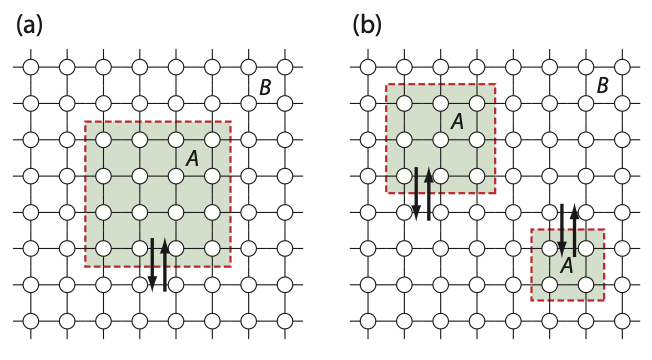
\includegraphics[width=0.8\textwidth]{Square_Lattice_Subsystems}
%	\end{figure}
	
	\begin{figure}[h]
		\centering
		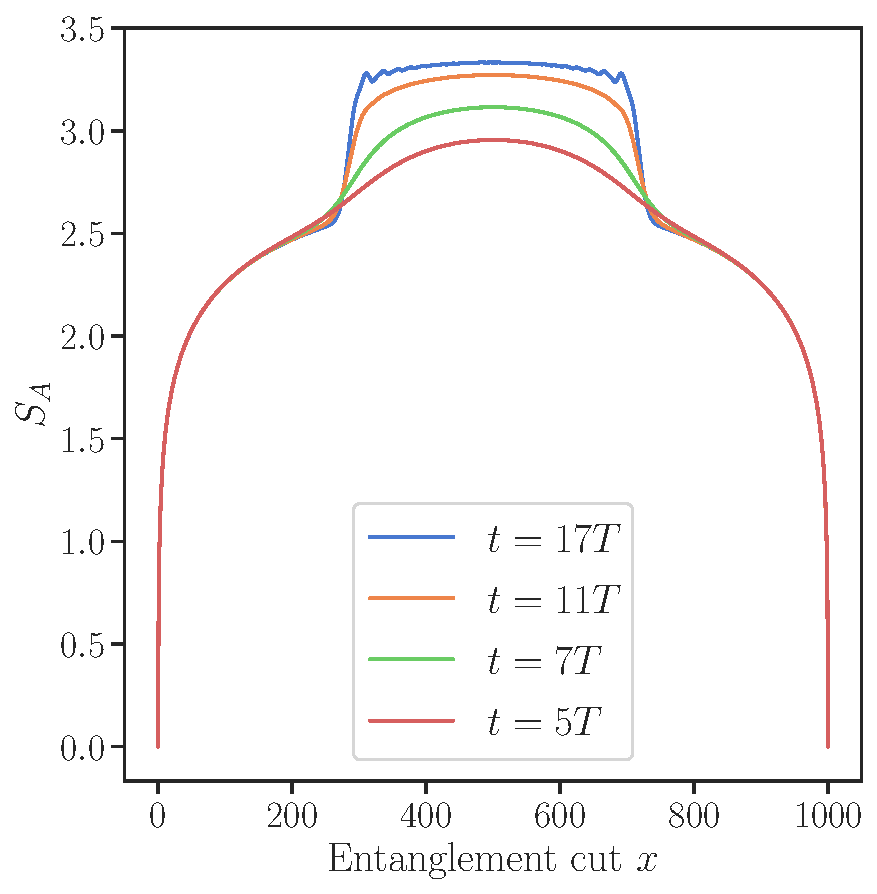
\includegraphics[width=0.8\textwidth]{Entanglement_Entropy}
		\caption{Evolution of the Entanglement Entropy of subsystem $A$ of a bipartite System as a function of the entanglement cut $x$ for stroboscopic measurements.}
		\label{}
	\end{figure}




	
	\section{Results} 
	
	
	\begin{figure}[h]
		\centering
		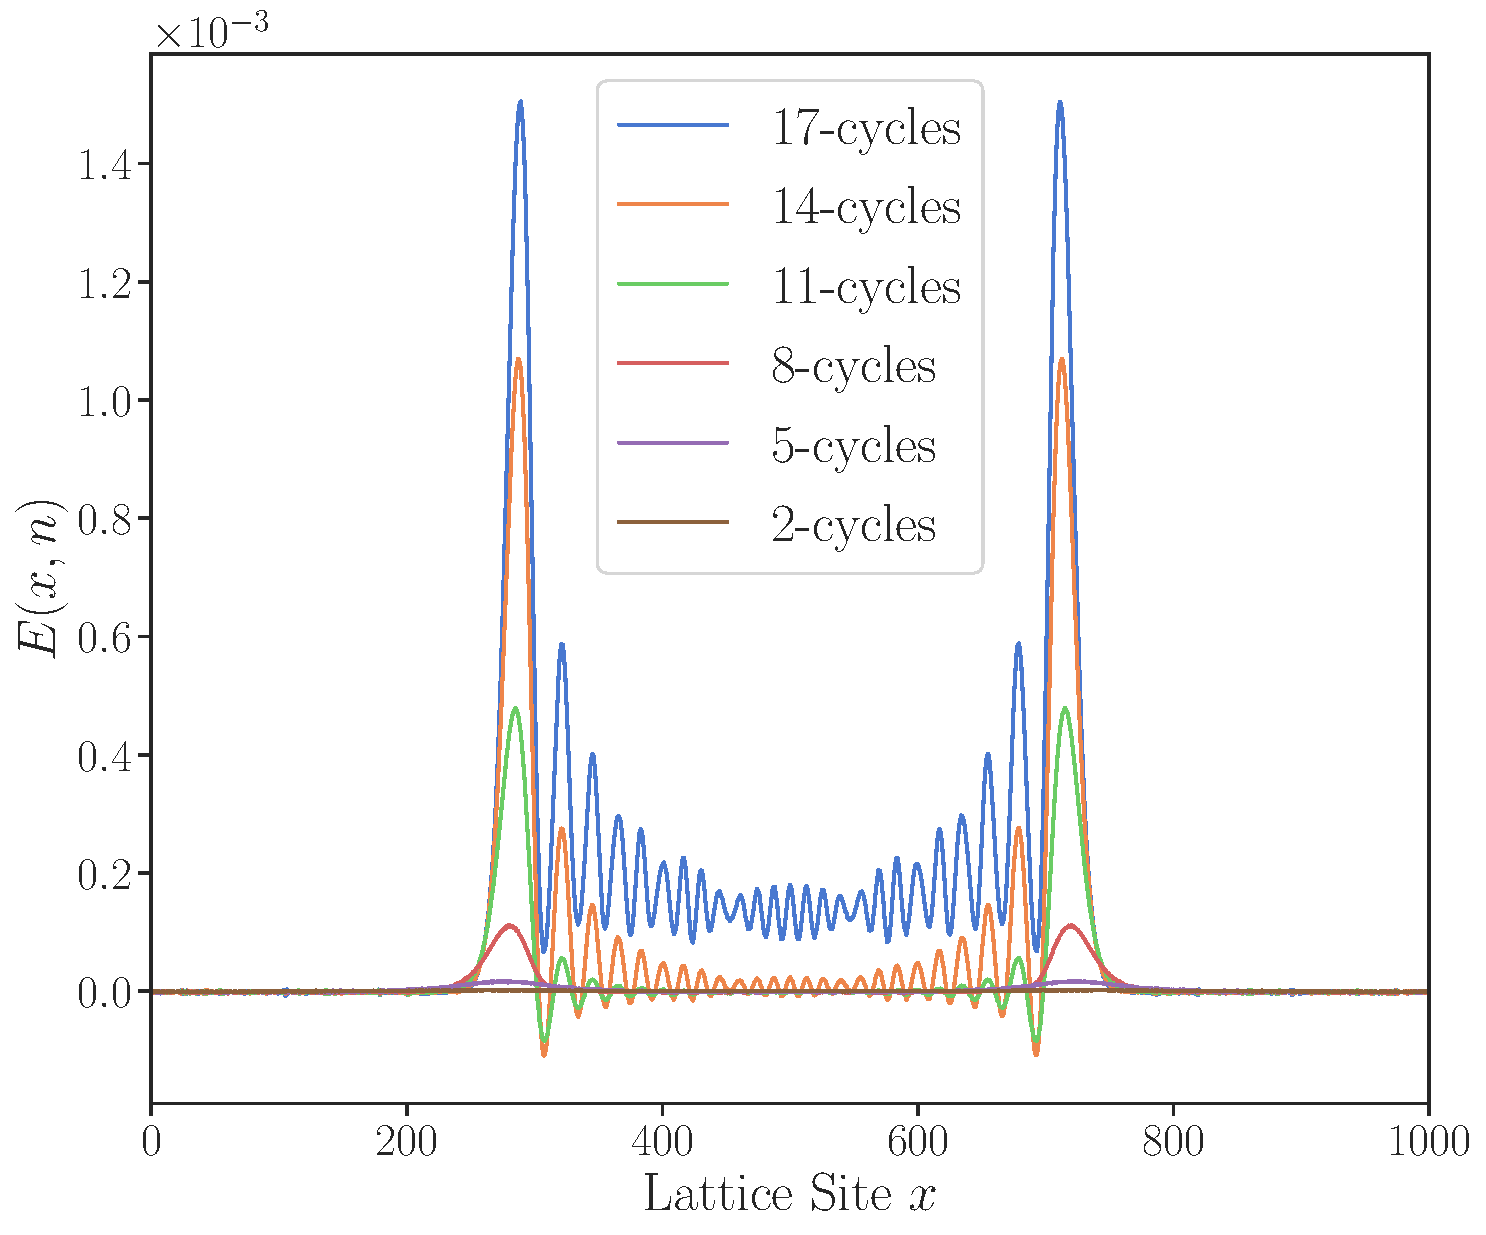
\includegraphics[width=0.8\textwidth]{Energy_Density1}
		\caption{Example of a \textit{heating phase} for a one-dimensional Floquet system of $L=1000$ lattice sites and driving parameters $T_0= 0.95L$ and $T_1 = 0.05L$ with Periodic Boundary Conditions}
	\end{figure}
	
	
	\begin{figure}[h]
	\centering
		\begin{subfigure}[b]{0.49\textwidth}
			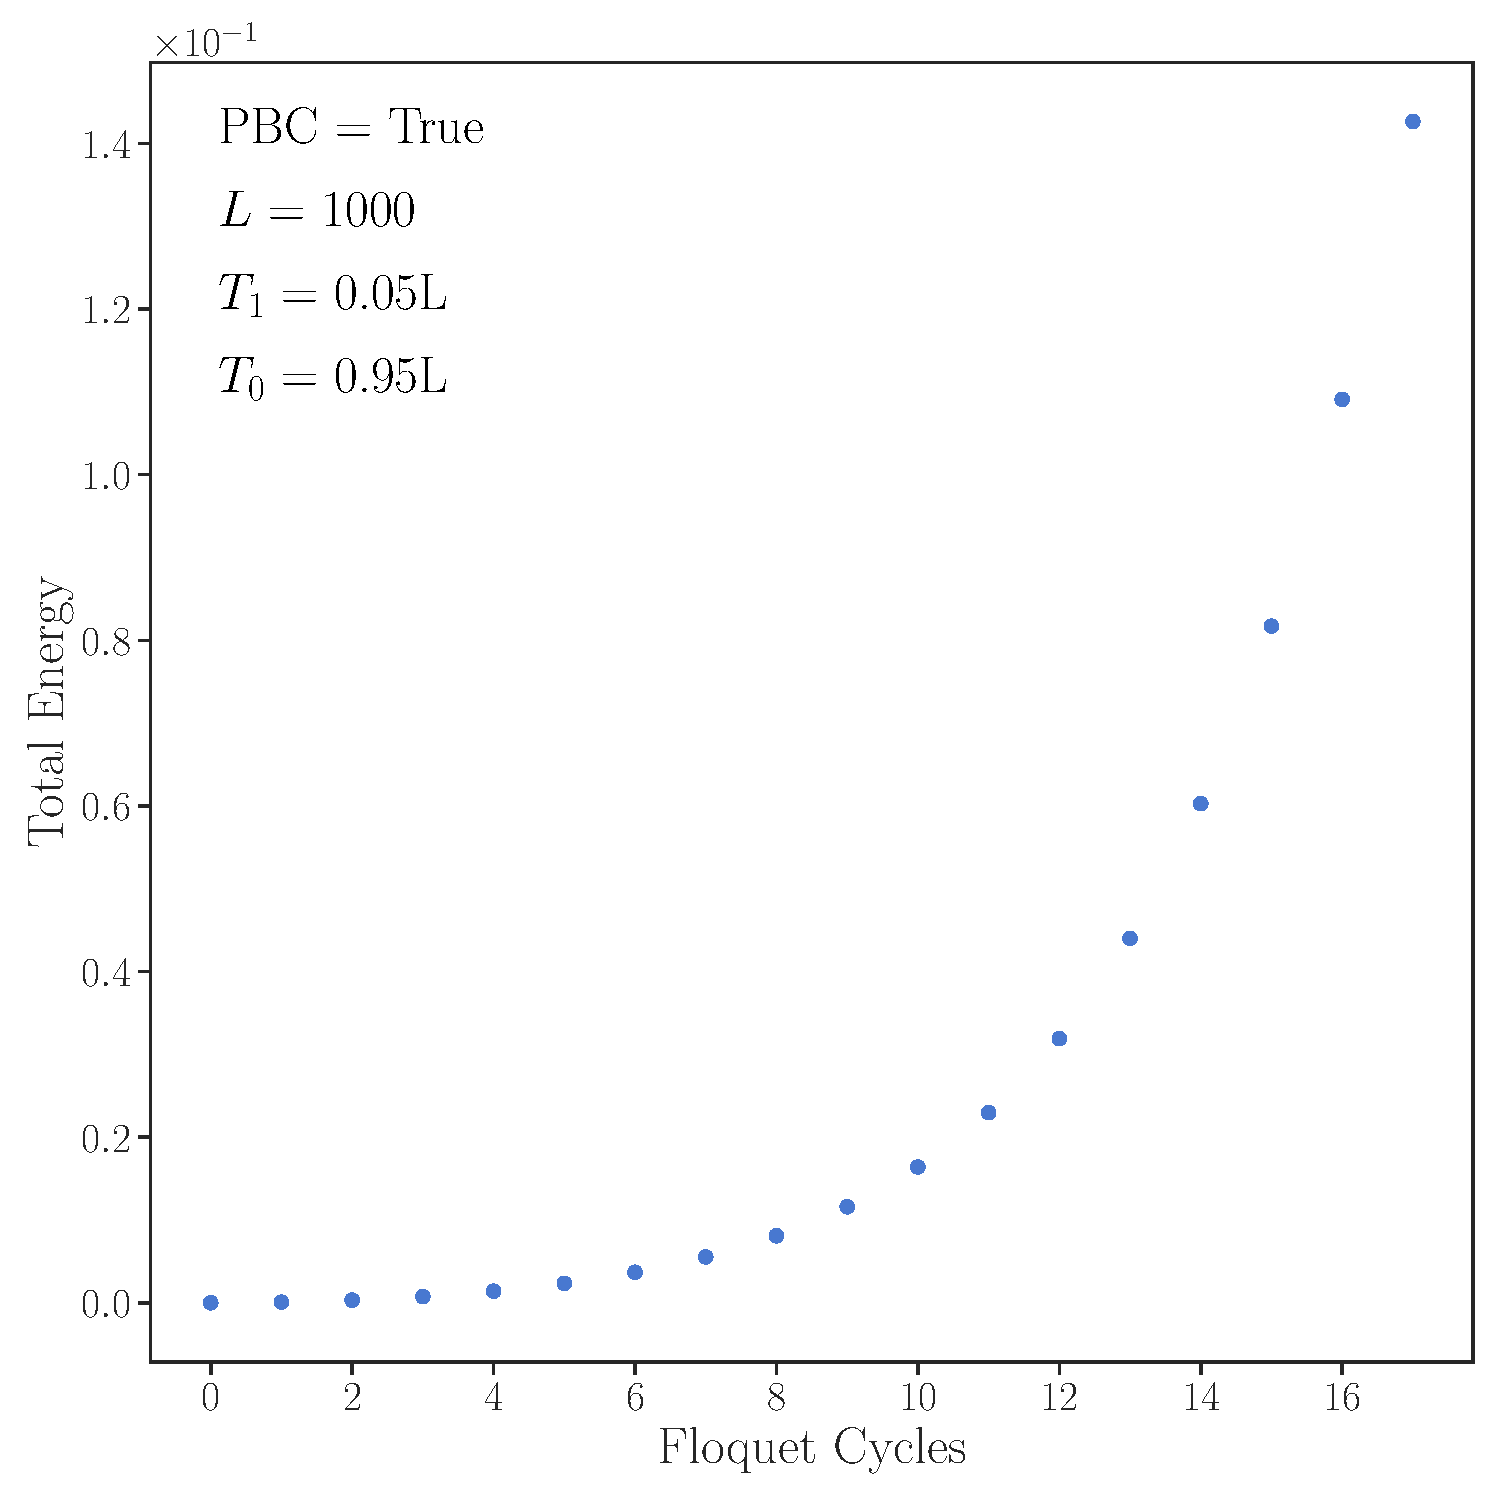
\includegraphics[width=\textwidth]{Total_Energy1d_heating.pdf}
		\end{subfigure}
		\begin{subfigure}[b]{0.49\textwidth}
			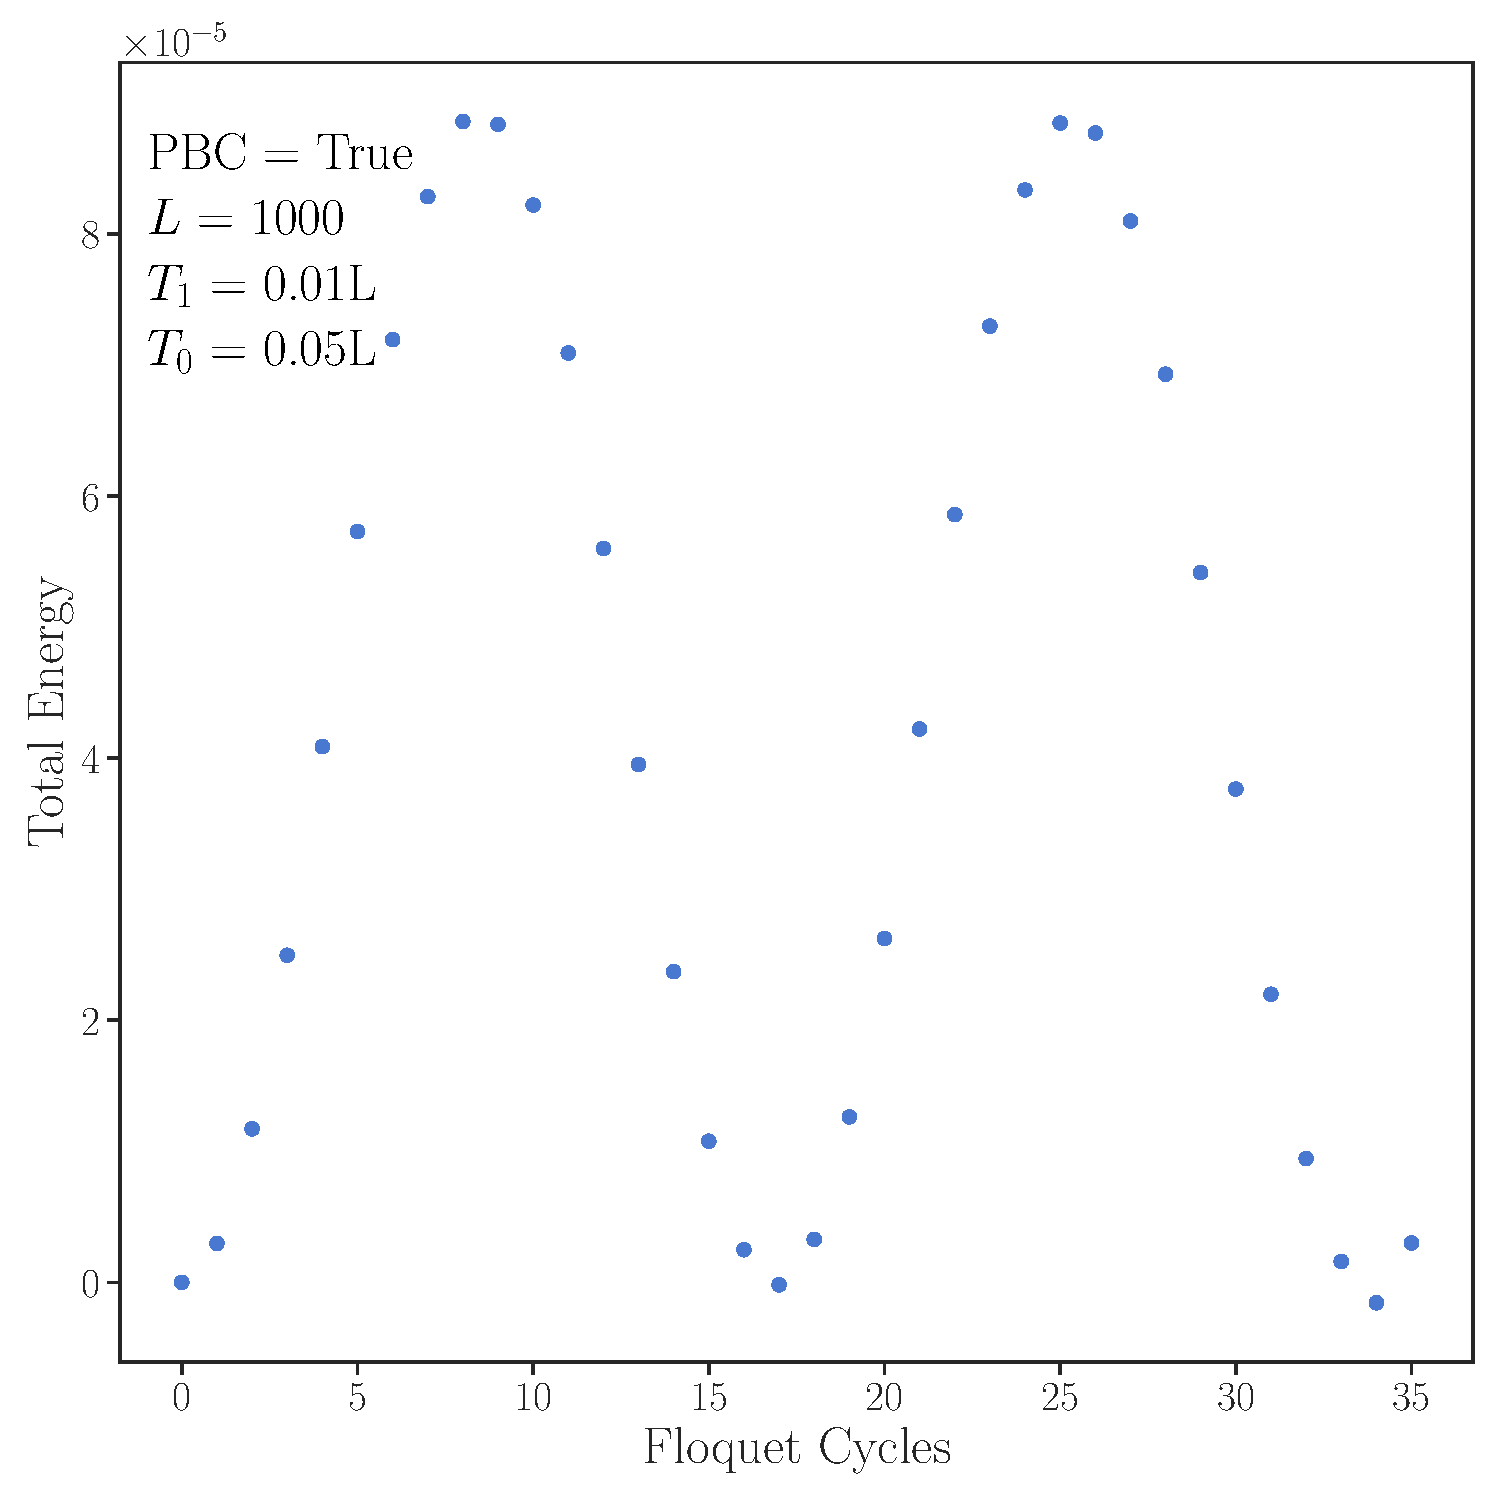
\includegraphics[width=\textwidth]{Total_Energy1d_nonheating.pdf}
		\end{subfigure}
		\caption{Total Energy for the (left) Heating Phase (right) Non-heating Phase}
	\end{figure}	
	
%	\begin{figure}[h]
%		\centering
%		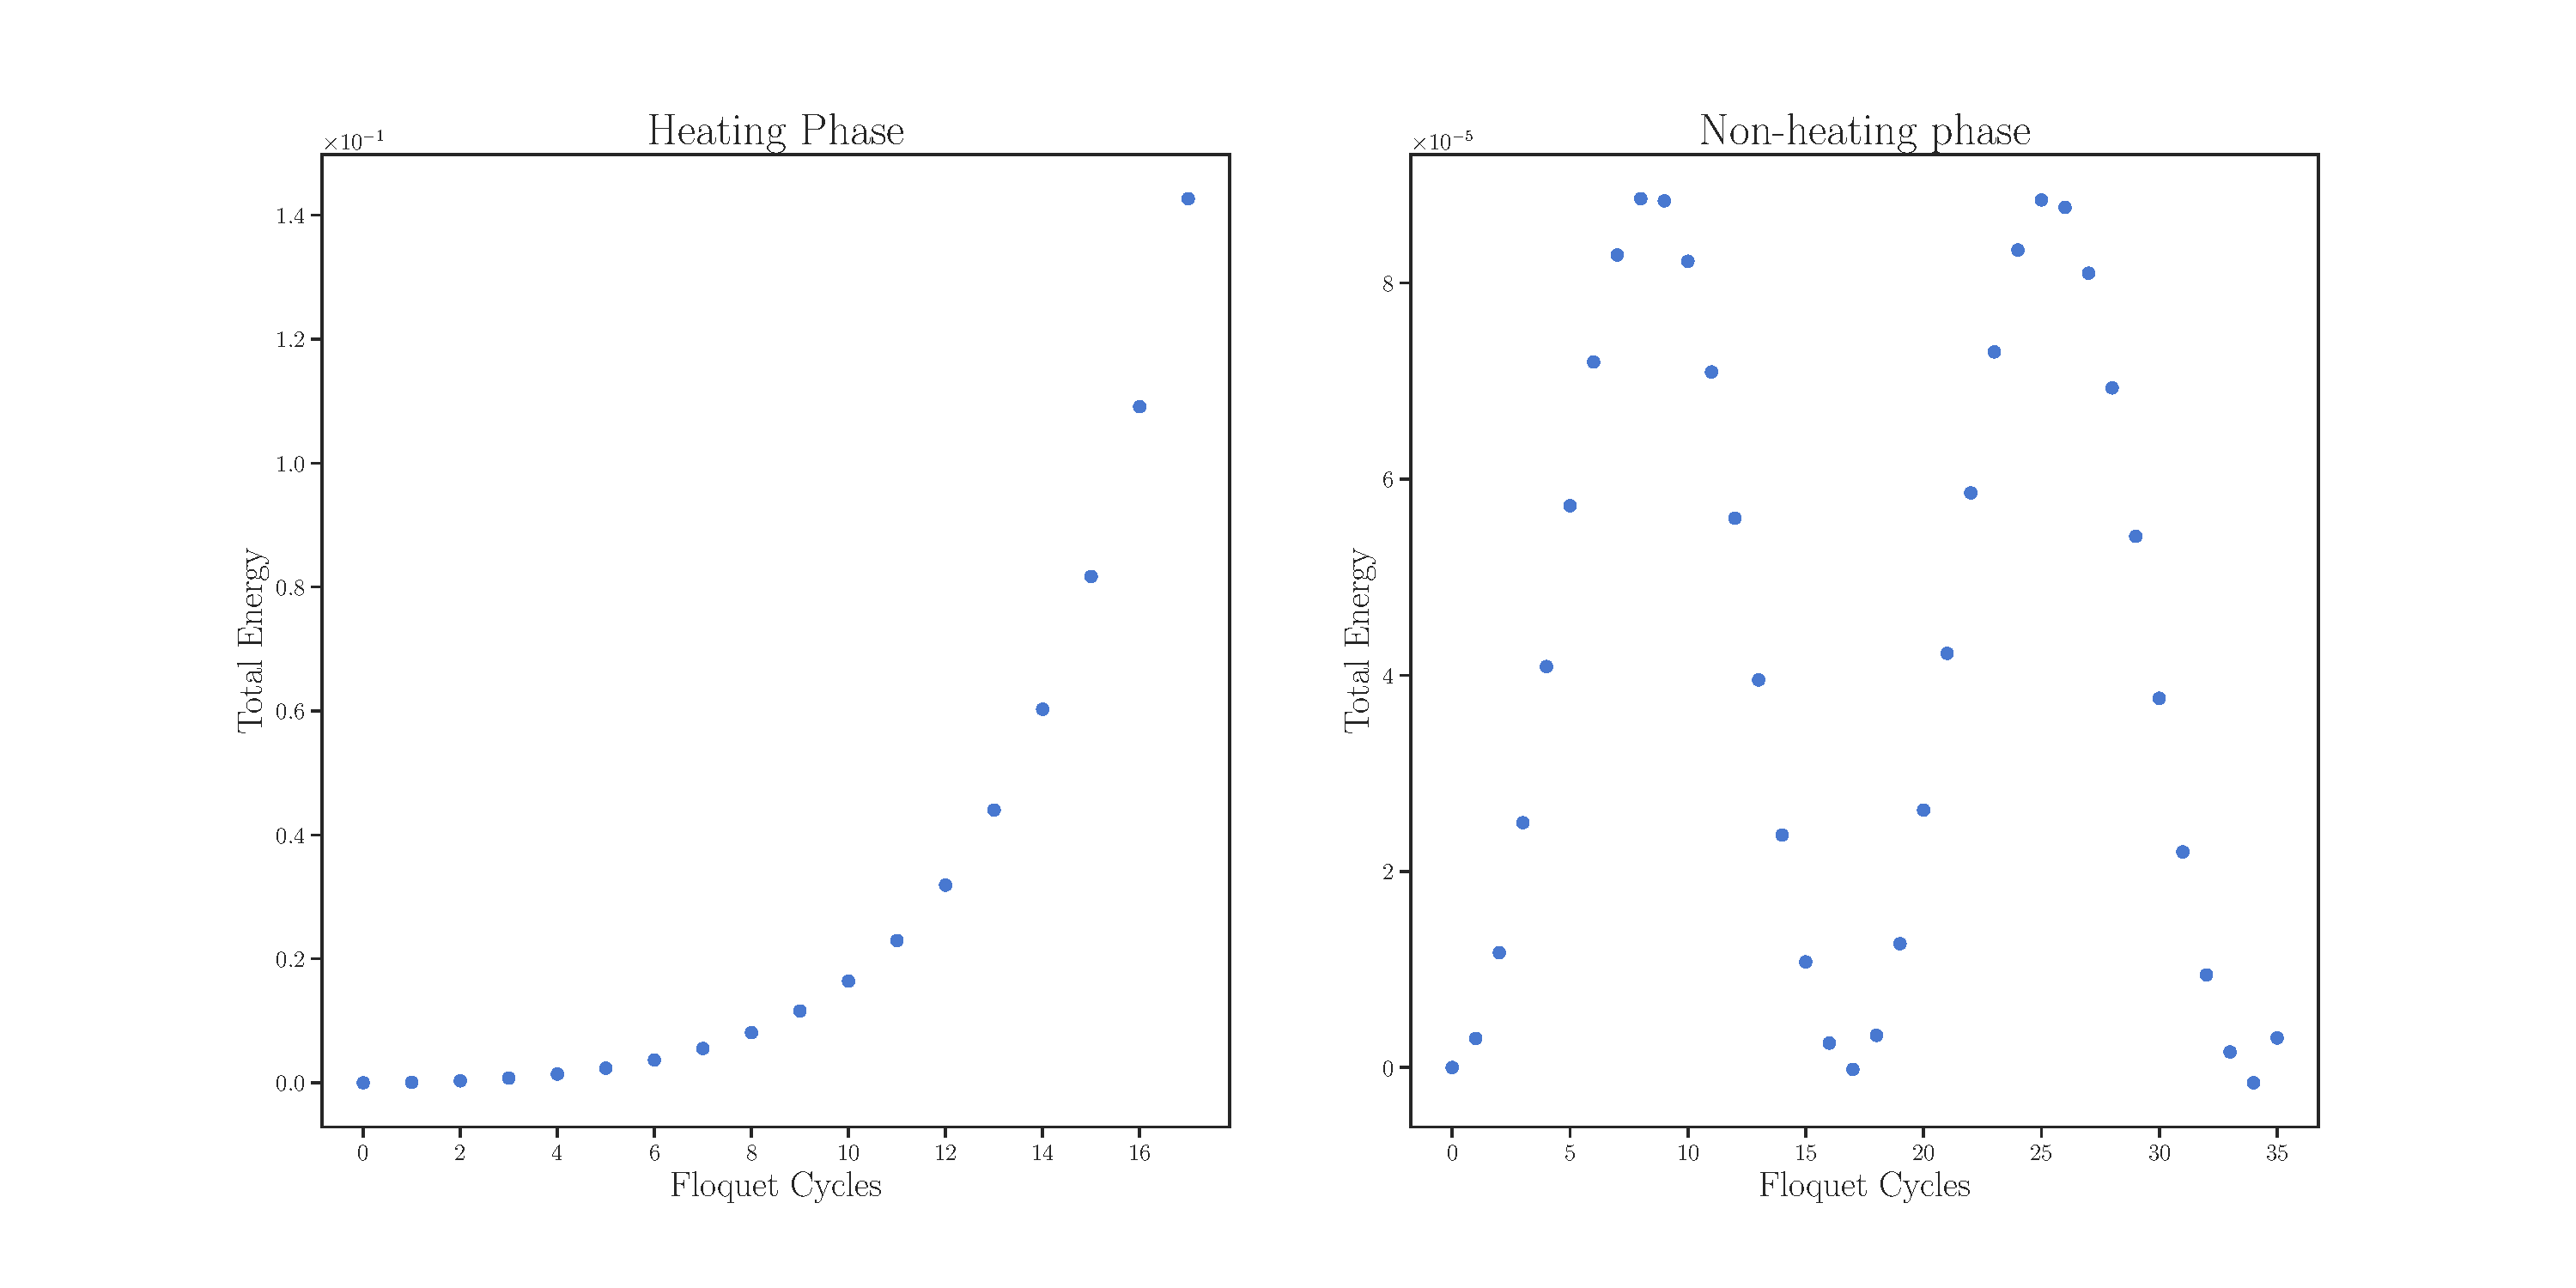
\includegraphics[width=\textwidth]{Total_Energy1d}
%		\caption{Structure of Total Energy over cycles of a non-heating and heating system}
%	\end{figure}
	
	\begin{figure}[h]
		\centering
		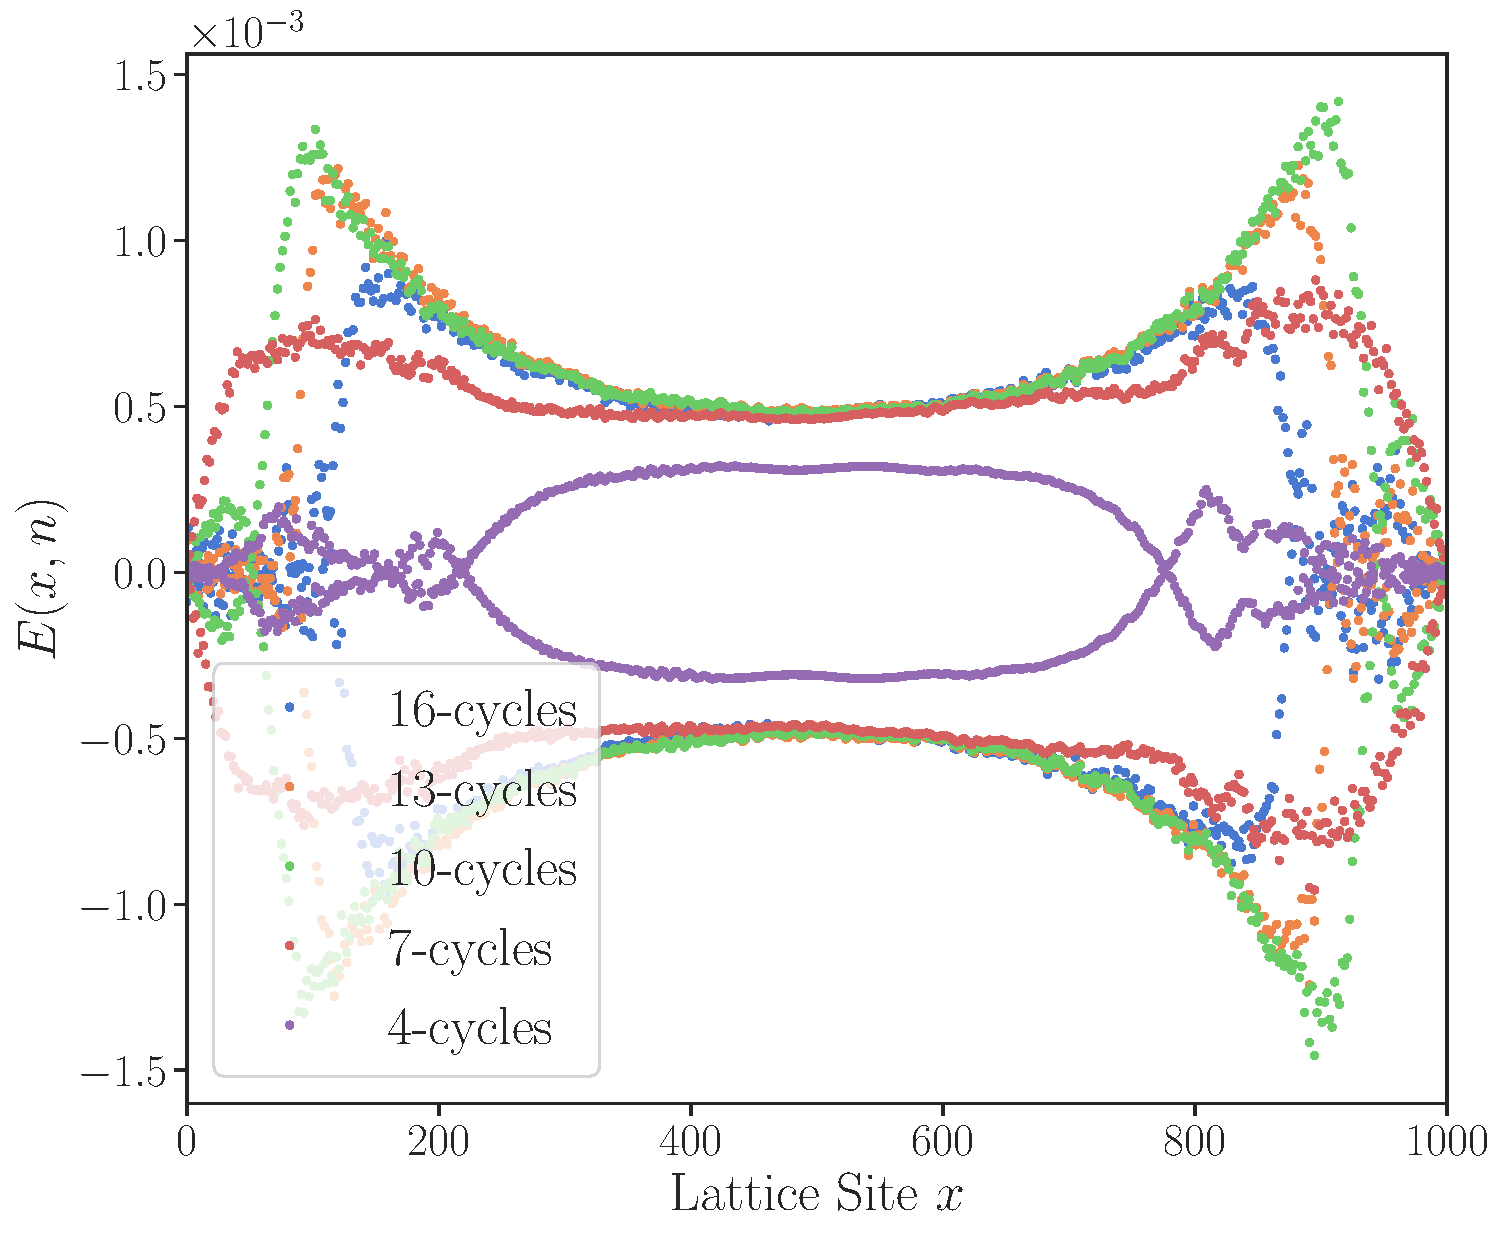
\includegraphics[width=0.8\textwidth]{Energy_Density2}
		\caption{Example of a \textit{non-heating} phase for a one-dimensional Floquet System of $L=1000$ lattices sites with driving parameters $T_0 = 0.2$ and $T_1 = 0.8$ and no Periodic Boundary Conditions}
	\end{figure}
	
	\section{Two-dimensional Floquet System}
	
	We will initially simply consider an extension of the tight-binding Hamiltonian in two-dimensions with only direct neighbor hopping meaning we consider
	\begin{equation}
		\mathcal{H}_0 = t_1\sum_{\vc{r}} [ \hat{c}^\dagger(x,y) \hat{c}(x+1, y) + \text{h.c}] + t_2\sum_{\vc{r}} [\hat{c}^\dagger(x,y) \hat{c}(x, y+1) + \text{h.c}]
	\end{equation}
	where $t_1$ and $t_2$ correspond to nearest-neighbor hopping in $x$ and $y$ directions respectively. Other than in the one-dimensional case we restrict ourself here to periodic-boundary conditions in both directions.
	
	
	This expresssion is best generalized as a sum over two indices. We best define the square lattice with the help of the coordinate tuple $(i, j)$ meaning our Hamiltonian takes the form
	\begin{equation}
		\hat{H}_0 =  \sum_{i = 1}^{L_x} \sum_{j=1}^{L_y} -\frac{t_1}{2} \left[ \hat{c}^\dagger(i, j) \hat{c}(i+1, j) + \hat{c}^\dagger(i+1, j)\hat{c}(i, j) \right] - \frac{t_2}{2} \left[\hat{c}^\dagger(i,j) \hat{c}(i,j+1) + \hat{c}^\dagger(i, j+1)\hat{c}(i,j) \right]
	\end{equation}
	
	\begin{figure}[h]	
		\centering
		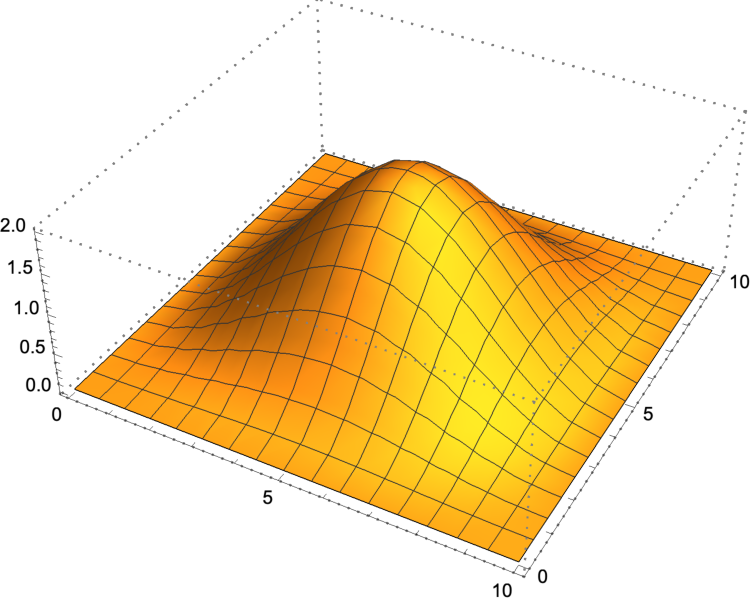
\includegraphics[width=0.6\textwidth]{chart2}
		\caption{Sine-Squared Deformation used in the two-dimensional Floquet Drive for a squared Lattice of $L=10$ sites}
	\end{figure}
	
	In an analog fashion to the one-dimensional case, we require to compute the Matrixelements of the Hamiltonian. In this case the creation and annihilation operators require two indices to properly define the state that is being acted on. We obtain the following expression for our matrix elements:
	\begin{equation}
		\mel{k,l}{\hat{H}_0}{m,n} = \mel{0}{\hat{c}(k,l)\hat{H}_0\hat{c}^\dagger(m,n)}{0} = t_2 \delta_{k,m}\delta_{l+1,n} + t_1 \delta_{k+1,m} \delta_{l,n} + t_2 \delta_{k,m} \delta_{l, n+1} + t_1 \delta_{k, m+1} \delta_{l,n}
	\end{equation}
	
	From now on we will label our single-particle basis $\ket{l,m}$ by a single index $\alpha$. Next we define the ordering of the states $(\alpha_1, \alpha_2, \dots)$ to be of normal ordering. Once this is agreed upon, we define the occupation number basis vectors $\ket{n_1, n_2, \dots}$. This means that for an $L \times L$ squared Lattice we obtain $L^2$ unique labels $\alpha$ for our basis states. In a similar manner we therefore define
	\begin{equation}
		\hat{c}_\alpha = \sum_\alpha \hat{U}_{\alpha \beta} b_\beta
	\end{equation}
	where $\alpha = (i,j)$ now implicitly sums over all possible combinations $(i,j)$ for $ i,j = 1, \dots N$. In a similar manner to the one-dimensional case we require the computation of the two-point correlation matrix where instead of obtaining $L$-eigenvectors and eigenvalues we get $L^2$ meaning our matrix $U$ is of the size $L^2 \times L^2$. \\
	
	
For our SSD Deformed Hamiltonian we use the following product
\begin{equation}
	\mathcal{F}(x,y) = f_x(x)f_y(y) = 4\sin(\frac{\pi x}{L})^2\sin(\frac{\pi y}{L})^2
\end{equation}
and the Sine-squared Hamiltonian takes the form
\begin{equation}
\begin{split}
\hat{H}_\text{SSD} = \sum_{i=1}^{L_x} \sum_{j=1}^{L_y} &t_1 \mathcal{F}\left(x+\frac{1}{2}, y\right) \left[ \hat{c}^\dagger(x,y)\hat{c}(x+1, y) + \hat{c}^\dagger(x+1,y) \hat{c}(x,y)\right] \\
&+ t_2 \mathcal{F}\left(x, y+ \frac{1}{2}\right) \left[\hat{c}^\dagger(x, y) \hat{c}(x, y + 1) + \hat{c}^\dagger(x, y+1) \hat{c}(x,y) \right]
\end{split}
\end{equation}
Which we will formulate with the help over a sum over two indices $i$ and $j$:
\begin{equation}
	\begin{split}
		\hat{H}_\text{SSD} = \sum_{i=1}^{L_x} \sum_{j=1}^{L_y} &t_1 \mathcal{F}\left(i+\frac{1}{2}, j\right) \left[ \hat{c}^\dagger(i,j)\hat{c}(i+1, j) + \hat{c}^\dagger(i+1,j) \hat{c}(i,j)\right] \\
&+ t_2 \mathcal{F}\left(i, j + \frac{1}{2}\right) \left[\hat{c}^\dagger(i, j) \hat{c}(i, j + 1) + \hat{c}^\dagger(i, j+1) \hat{c}(i,j) \right]
	\end{split}
\end{equation}
	
%	For the deformed Hamiltonian we first simply assume an arbitrary deformation of the form
%	\begin{equation}
%		\hat{H}_\text{SSD} = - \frac{t
%	\end{equation}	\subsection{Designing the Sine-Squared Deformed Hamiltonian}
	- Perron-Frobenius theorem: enables us to prove that the Fermi sea is the ground state of the SSD Hamiltonian
	- In higher dimensions, it is in general impossible to find a basis in which all of the off-diagonal elements of the Hamiltonian are non-positive due to fermion signs.
	- Therefore the ground state of the SSD Hamiltonian is not necessarily the Fermi sea of the periodic system.
	
	\begin{figure}[h]
		\begin{subfigure}[c]{0.45\textwidth}
			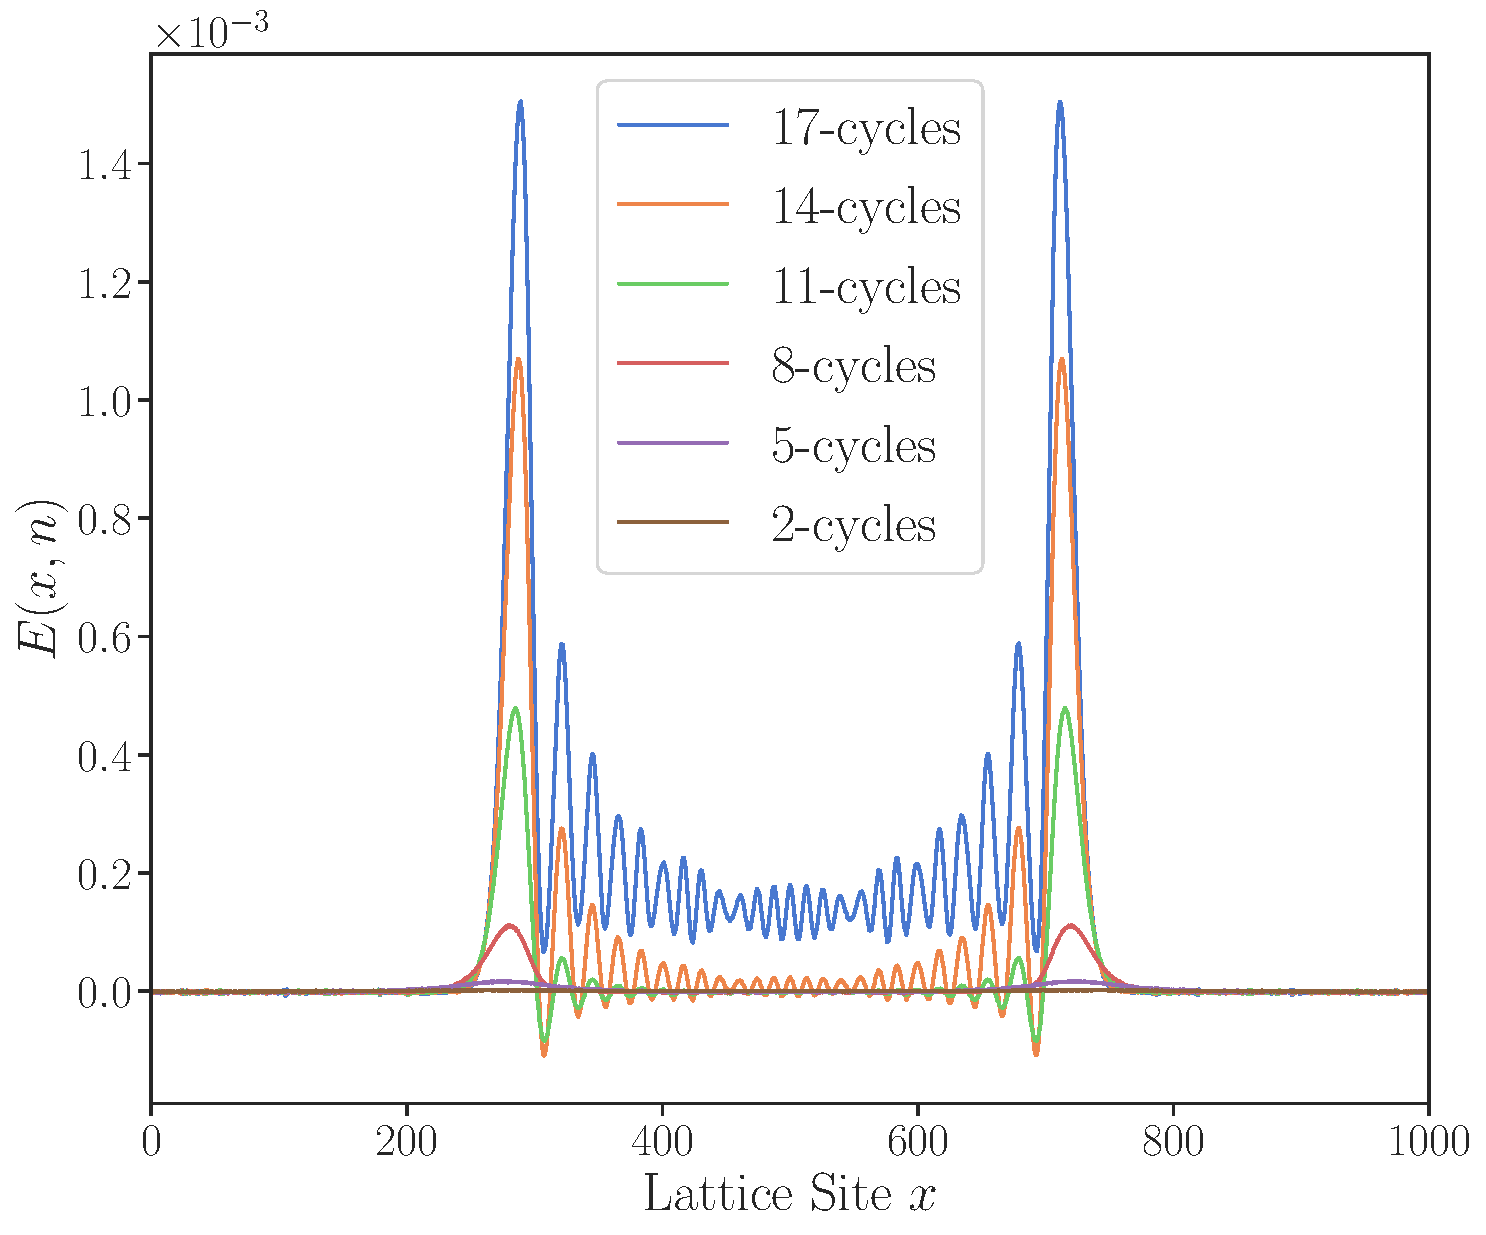
\includegraphics[width=\textwidth]{Energy_Density1}
		\end{subfigure}
		\begin{subfigure}[c]{0.45\textwidth}
			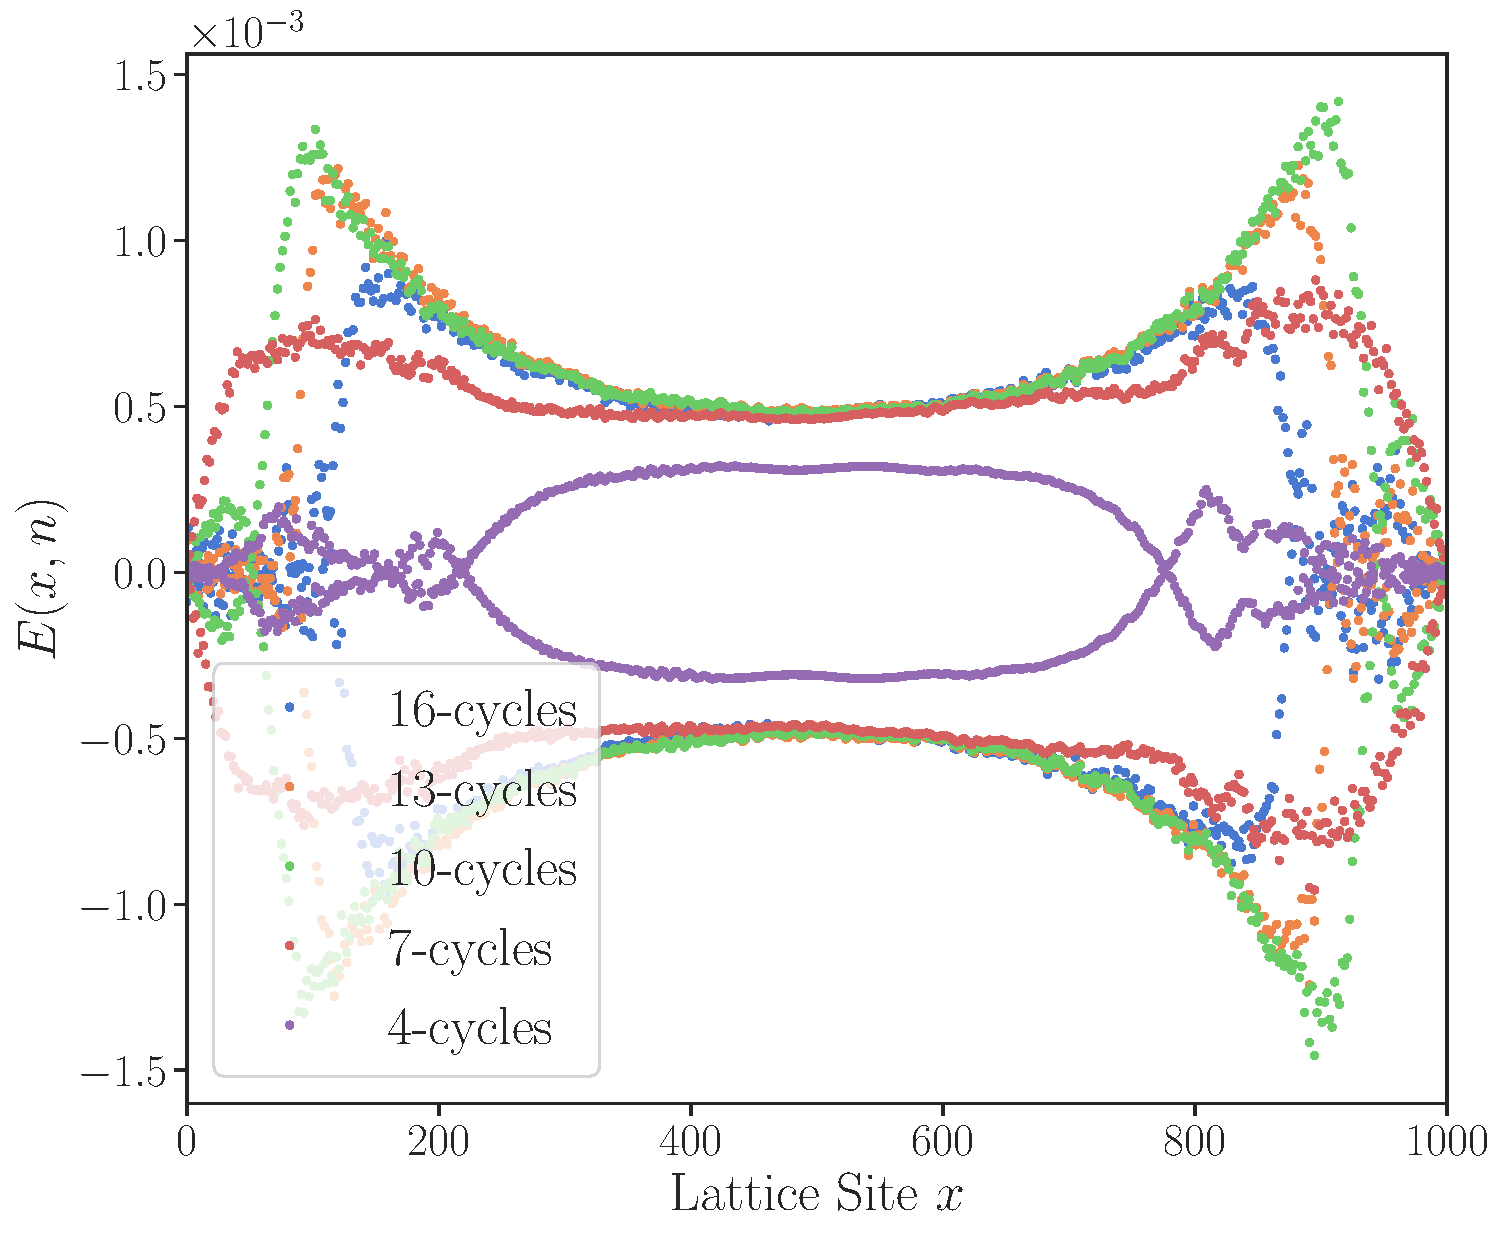
\includegraphics[width=\textwidth]{Energy_Density2}
		\end{subfigure}
		\caption{}
	\end{figure}
	
	
	
	\begin{figure}[h]
		\centering
		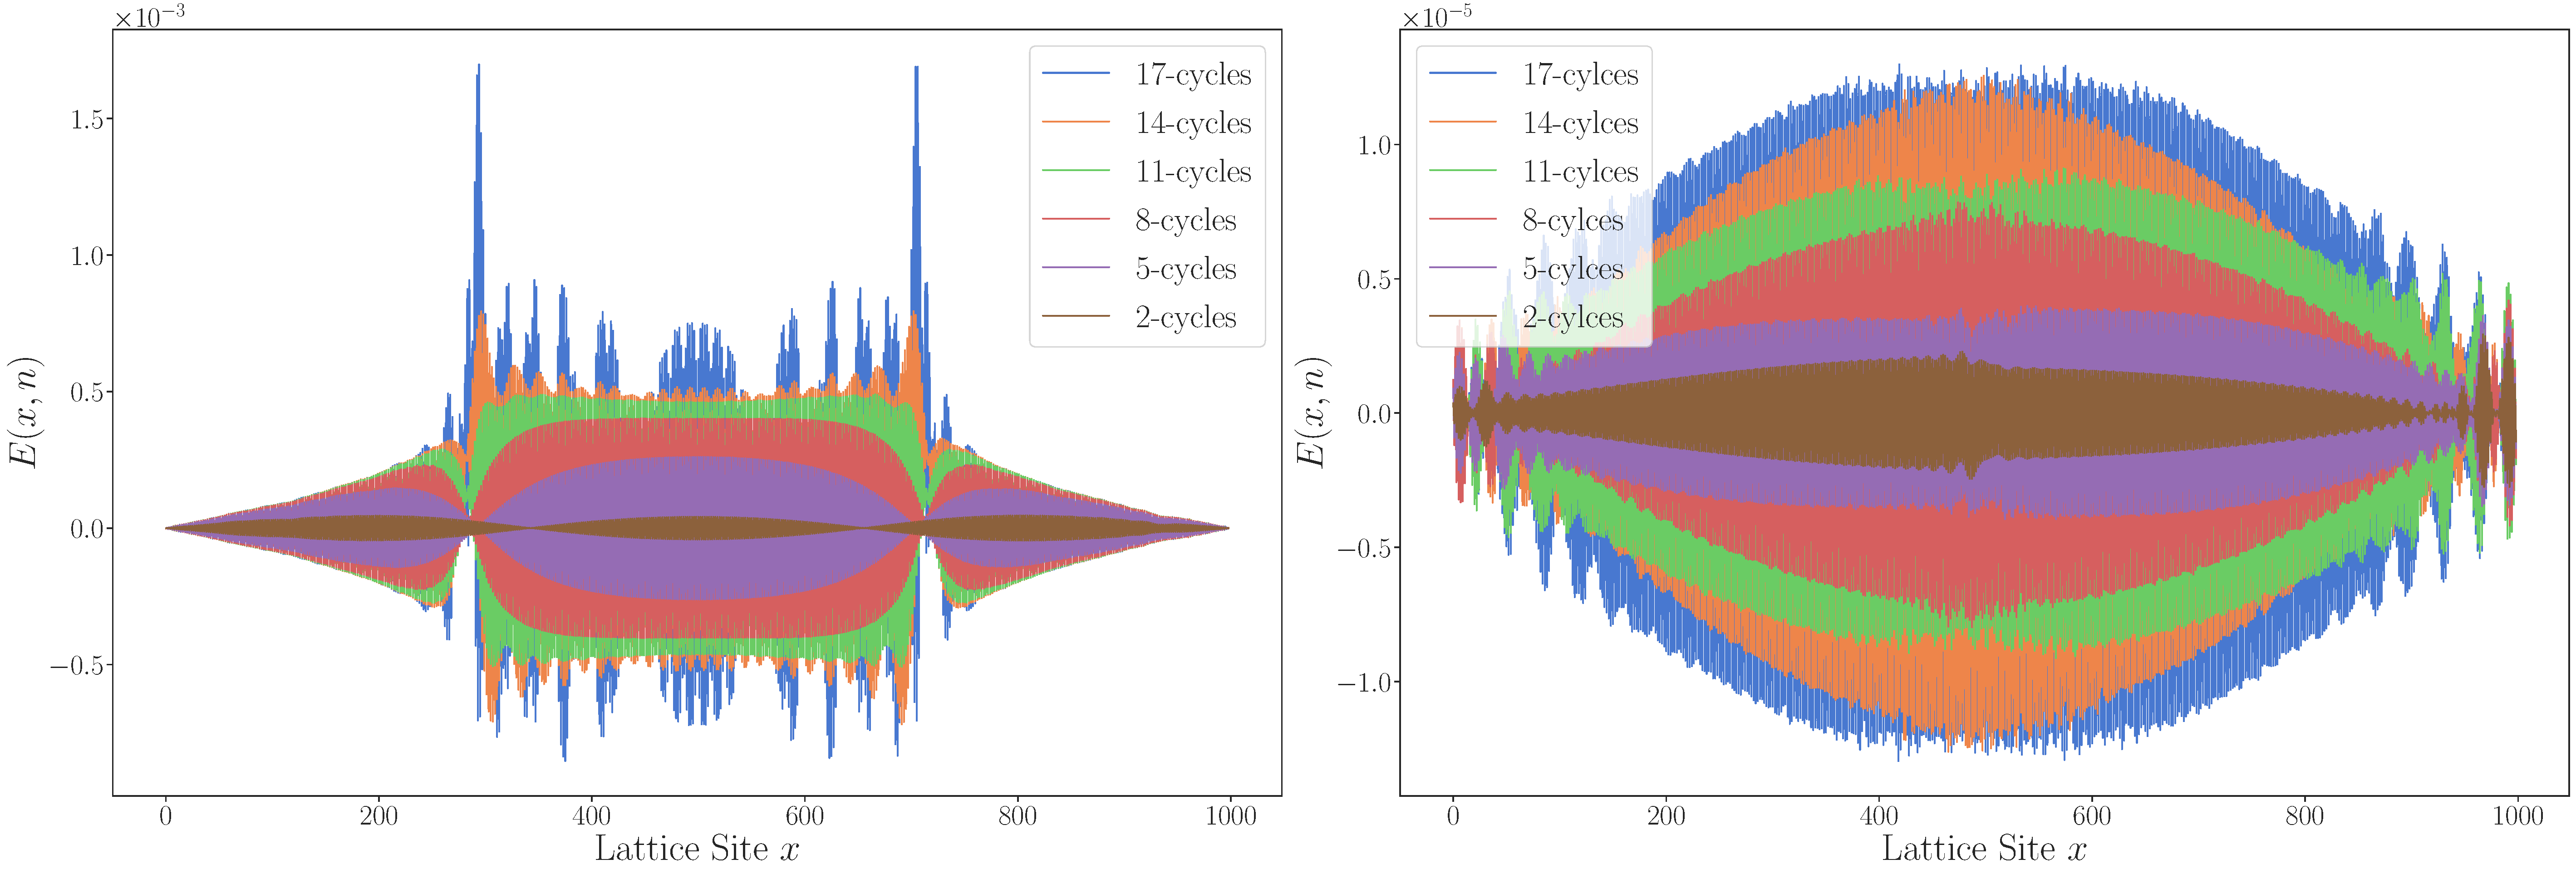
\includegraphics[width=\textwidth]{Energy_Density_Combined_OBC}
		\caption{Heating and non-heating phase of a system with \textit{Open Boundary Condition} and $L=1000$ with Parameters $T_0 = 0.95, T_1 = 0.05$ for the heating phase and $T_0 = 0.5$ and $T_1 = 0.01$}
	\end{figure}
	
	\begin{figure}[h]
		\centering
		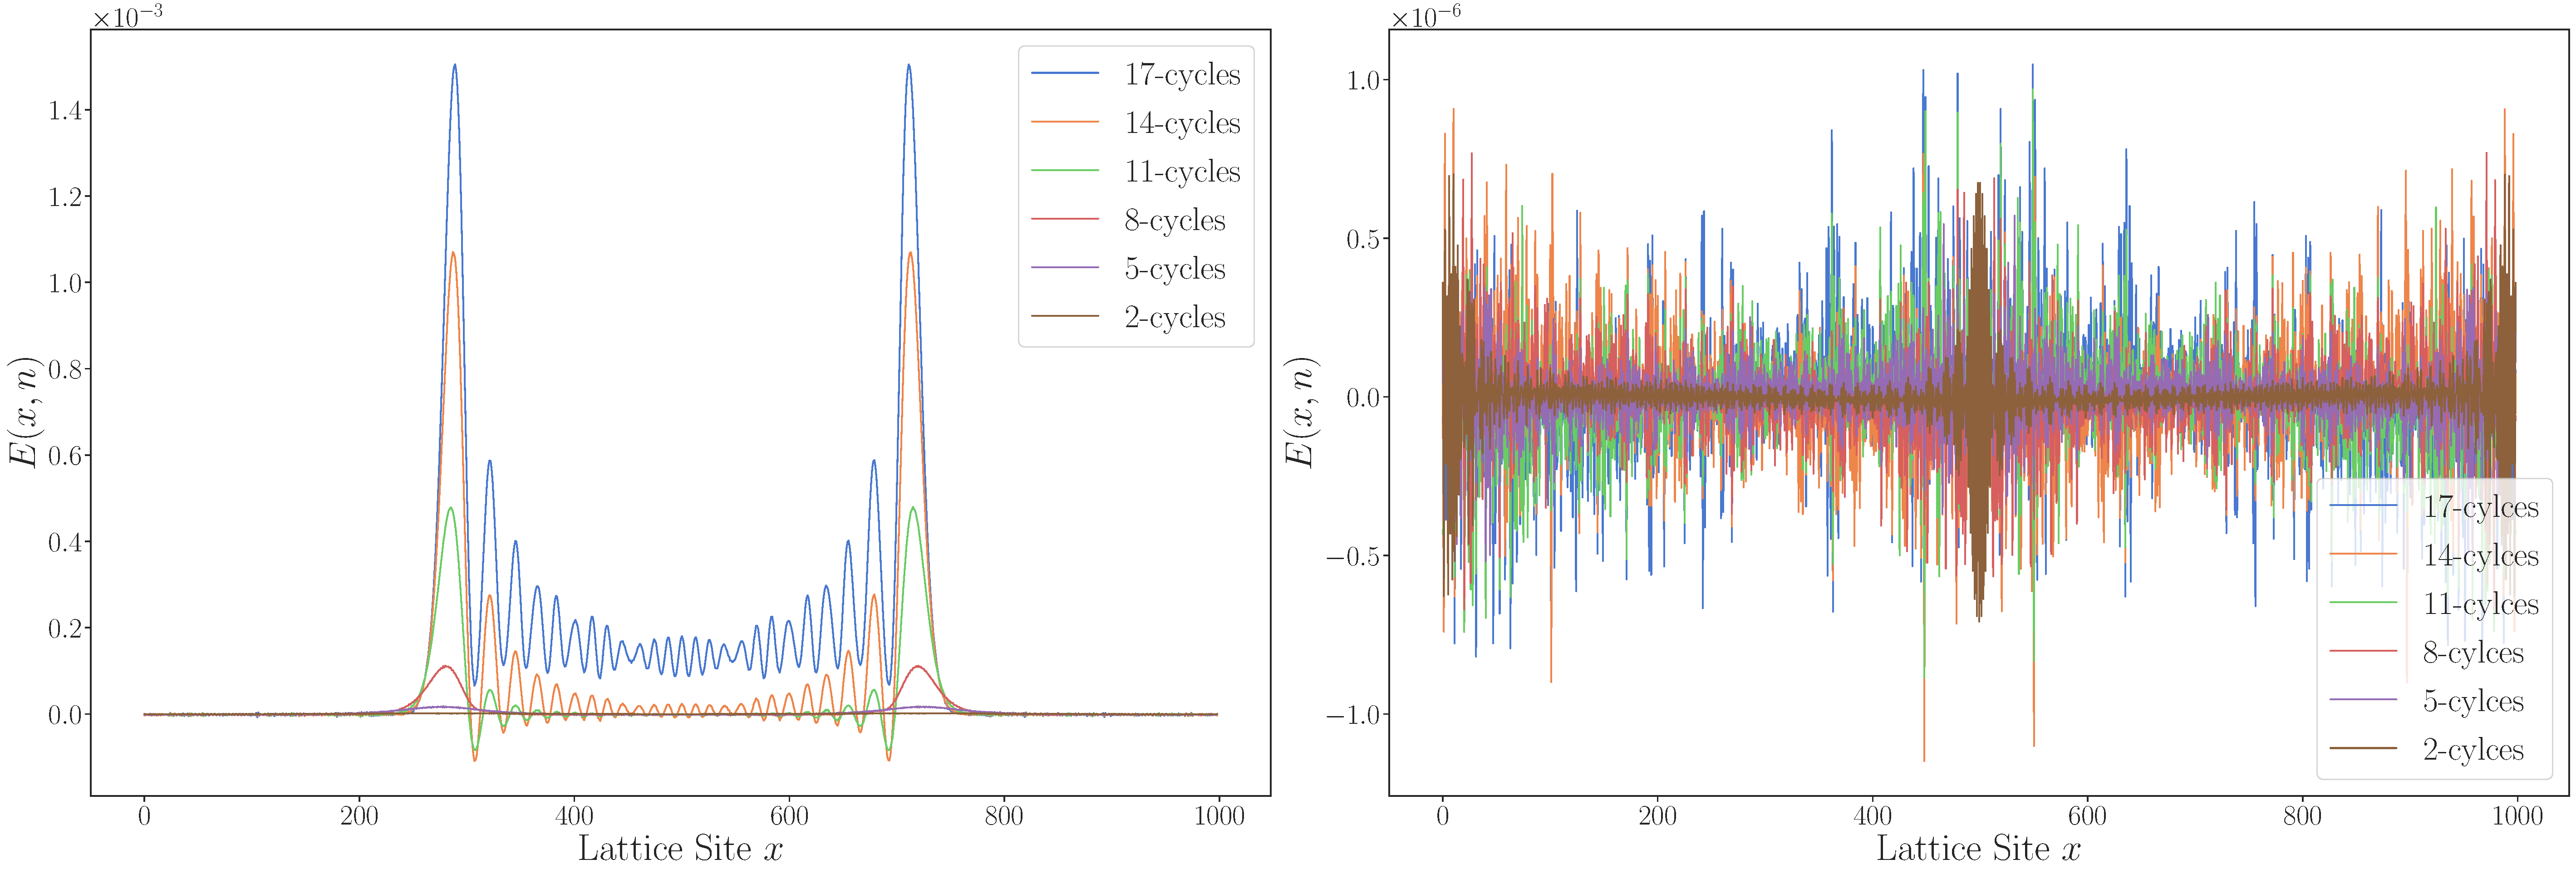
\includegraphics[width =\textwidth]{Energy_Density_Combined_PBC}
		\caption{Heating and non-heating phase of a system with \textit{Periodic Boundary Condition} and $L=1000$ with Parameters $T_0 = 0.95, T_1 = 0.05$ for the heating phase and $T_0 = 0.5$ and $T_1 = 0.01$}
	\end{figure}
	
	

\section{Results}

In the heating phase, although the total energy and entanglement keep growing, the system does not evolve into a featureless state. We find that, in this phase, the system heats up in a very nonuniform way. The energy pumped in concentrates at two points, one of which has purely chiral excitations and the other one has only antichiral excitations. The entanglement entropy also comes from the entanglement between the excitations at these two points. Furthermore, the energy and entanglement entropy are related by a simple formula. All these features above are universal and depend only on the central charge of the CFT. In the nonheating phase, if we do a stroboscopic measurement, we can find that energy excitation will move back and forth in the system with the total energy and entanglement entropy oscillating in time.
	
	
\printbibliography[heading=bibintoc,title={Bibliography}]

\end{document}
